% ============================================================================
% Rapport de stage - Cycle Ingénieur ESPRIT
% Assistant IA e-commerce & Backoffice - Prodexo
% ============================================================================
%
% Compilation : pdflatex main.tex && pdflatex main.tex && makeglossaries main && pdflatex main.tex
% (ou tectonic main.tex, testé pendant la rédaction de ce rapport)
%
% NOTE : ce document utilise une page de garde générique. Si ESPRIT fournit
% une classe officielle (esprit.cls) ou un template de page de garde avec
% logos, remplacez le contenu de chapitres/00_page_garde.tex par le template
% officiel plutôt que d'adapter celui-ci.
% ============================================================================

\documentclass[12pt, a4paper, oneside]{report}

% --- Encodage et langue ---
\usepackage[utf8]{inputenc}
\usepackage[T1]{fontenc}
\usepackage[french]{babel}
\usepackage{lmodern}
% NOTE : ce document utilise \oe{} plutôt que le caractère "\oe{}" littéral, pour
% rester compilable aussi bien avec pdflatex qu'avec XeTeX/LuaTeX (tectonic).

% --- Mise en page ---
\usepackage[a4paper, left=3cm, right=2.5cm, top=2.5cm, bottom=2.5cm]{geometry}
\usepackage{setspace}
\onehalfspacing
\usepackage{fancyhdr}
\usepackage{titlesec}
\usepackage{emptypage}

% --- Graphismes et couleurs ---
\usepackage{graphicx}
\usepackage{xcolor}
\definecolor{esprit_bordeaux}{RGB}{130,0,20}
\definecolor{prodexo_bleu}{RGB}{20,60,110}
\definecolor{codegray}{RGB}{245,245,245}

% --- Tableaux ---
\usepackage{array}
\usepackage{booktabs}
\usepackage{longtable}
\usepackage{multirow}
\usepackage{colortbl}

% --- Listes et code ---
\usepackage{enumitem}
\usepackage{listings}
\lstset{
  backgroundcolor=\color{codegray},
  basicstyle=\ttfamily\footnotesize,
  breaklines=true,
  frame=single,
  numbers=left,
  numberstyle=\tiny\color{gray},
  keywordstyle=\color{prodexo_bleu}\bfseries,
  commentstyle=\color{gray}\itshape,
  stringstyle=\color{esprit_bordeaux},
  showstringspaces=false,
  tabsize=2,
  captionpos=b,
}

% --- Mathématiques (chargé avant cleveref, requis par ce dernier) ---
\usepackage{amsmath}

% --- Liens et références ---
\usepackage{hyperref}
\hypersetup{
  colorlinks=true,
  linkcolor=prodexo_bleu,
  citecolor=prodexo_bleu,
  urlcolor=prodexo_bleu,
  pdftitle={Rapport de stage - Assistant IA e-commerce et Backoffice},
  pdfauthor={Oussama Wannassi},
}
\usepackage[capitalize]{cleveref}

% --- Bibliographie ---
% NOTE : bibliographie gérée manuellement (\chapter*{Bibliographie et Netographie}
\addcontentsline{toc}{chapter}{Bibliographie et Netographie}
\markboth{Bibliographie et Netographie}{}

\begin{thebibliography}{99}

\bibitem{scrumguide}
Schwaber, K. et Sutherland, J. \emph{The Scrum Guide}. 2020.
\url{https://scrumguides.org/}

\bibitem{fastapi}
\emph{FastAPI Documentation}. 2026.
\url{https://fastapi.tiangolo.com/}

\bibitem{sqlalchemy}
\emph{SQLAlchemy 2.0 Documentation}. 2026.
\url{https://docs.sqlalchemy.org/en/20/}

\bibitem{filament}
\emph{Filament -- Rapid Laravel Development Framework}. 2026.
\url{https://filamentphp.com/docs}

\bibitem{livewire}
\emph{Laravel Livewire Documentation}. 2026.
\url{https://livewire.laravel.com/docs}

\bibitem{chromadb}
\emph{Chroma -- The AI-native Open-source Embedding Database}. 2026.
\url{https://docs.trychroma.com/}

\bibitem{owasp-llm}
OWASP Foundation. \emph{OWASP Top 10 for Large Language Model Applications}. 2025.
\url{https://owasp.org/www-project-top-10-for-large-language-model-applications/}

\bibitem{c4model}
Brown, S. \emph{The C4 model for visualising software architecture}. 2026.
\url{https://c4model.com/}

\bibitem{prestashop-webservice}
\emph{PrestaShop Webservice API Documentation}. 2026.
\url{https://devdocs.prestashop-project.org/8/webservice/}

\bibitem{redis-docs}
\emph{Redis Documentation}. 2026.
\url{https://redis.io/docs/}

\end{thebibliography}
)
% plutôt que via biblatex+biber, pour rester compilable sans dépendance
% externe (biber accuse un décalage de version fréquent avec biblatex selon
% les distributions LaTeX). Les mêmes références restent disponibles au
% format .bib (bibliographie.bib) si vous préférez rebasculer sur biblatex.

% --- Acronymes / glossaire ---
\usepackage[toc, acronym]{glossaries}
\makeglossaries
% Liste des abréviations (chargée par \printglossary[type=\acronymtype] dans main.tex)

\newacronym{api}{API}{Application Programming Interface}
\newacronym{rag}{RAG}{Retrieval-Augmented Generation (génération augmentée par récupération de contexte)}
\newacronym{llm}{LLM}{Large Language Model (grand modèle de langage)}
\newacronym{crud}{CRUD}{Create, Read, Update, Delete}
\newacronym{orm}{ORM}{Object-Relational Mapping}
\newacronym{cicd}{CI/CD}{Continuous Integration / Continuous Deployment}
\newacronym{jsonb}{JSONB}{JSON Binary (type de données PostgreSQL)}
\newacronym{rest}{REST}{Representational State Transfer}
\newacronym{sql}{SQL}{Structured Query Language}
\newacronym{ttl}{TTL}{Time To Live}
\newacronym{cve}{CVE}{Common Vulnerabilities and Exposures}
\newacronym{sla}{SLA}{Service Level Agreement}
\newacronym{uuid}{UUID}{Universally Unique Identifier}
\newacronym{pii}{PII}{Personally Identifiable Information (données à caractère personnel)}
\newacronym{http}{HTTP}{HyperText Transfer Protocol}
\newacronym{pfe}{PFE}{Projet de Fin d'Études}
\newacronym{wal}{WAL}{Write-Ahead Logging}


% --- En-têtes / pieds de page ---
\pagestyle{fancy}
\fancyhf{}
\renewcommand{\headrulewidth}{0.4pt}
\fancyhead[L]{\small\leftmark}
\fancyhead[R]{\small Rapport de stage -- Oussama Wannassi}
\fancyfoot[C]{\thepage}

\titleformat{\chapter}[display]
  {\normalfont\huge\bfseries\color{prodexo_bleu}}
  {\chaptertitlename\ \thechapter}{20pt}{\Huge}
\titlespacing*{\chapter}{0pt}{0pt}{40pt}

\begin{document}

% ----------------------------------------------------------------------------
% Pages liminaires
% ----------------------------------------------------------------------------
\pagenumbering{roman}

% ----------------------------------------------------------------------------
% Page de garde
% NOTE : remplacer par le template officiel ESPRIT (logos ESPRIT + Prodexo,
% mentions obligatoires) si disponible. Les champs entre [ ] sont à compléter.
% ----------------------------------------------------------------------------
\begin{titlepage}
\centering

% \includegraphics[width=4cm]{images/logo_esprit.png} \hfill \includegraphics[width=4cm]{images/logo_prodexo.png}
{\large \textbf{Ecole Supérieure Privée d'Ingénierie et de Technologies -- ESPRIT}\par}
\vspace{0.3cm}
{\normalsize Département : Génie Informatique -- Cycle Ingénieur\par}

\vspace{2.5cm}
\rule{\linewidth}{1pt}\par
\vspace{0.6cm}
{\huge \bfseries Conception et développement d'un assistant conversationnel IA e-commerce et de son backoffice d'administration\par}
\vspace{0.6cm}
\rule{\linewidth}{1pt}\par

\vspace{1.5cm}
{\Large Rapport de stage\par}
\vspace{0.3cm}
{\normalsize présenté en vue de l'obtention du diplôme national d'ingénieur\par}

\vspace{2cm}

\begin{minipage}{0.45\textwidth}
\begin{flushleft} \large
\textbf{Élaboré par :}\\
Oussama Wannassi
\end{flushleft}
\end{minipage}
\begin{minipage}{0.45\textwidth}
\begin{flushright} \large
\textbf{Encadré par :}\\
Encadrant académique (ESPRIT) : [Nom à compléter]\\
Encadrant professionnel (Prodexo) : [Nom à compléter]
\end{flushright}
\end{minipage}

\vspace{2cm}

{\normalsize \textbf{Entreprise d'accueil :} Prodexo\par}
{\normalsize \textbf{Période de stage :} du 01/02/2026 au 01/08/2026\par}

\vfill

{\normalsize Année universitaire 2025 -- 2026\par}

\end{titlepage}

\newpage
\thispagestyle{empty}
\mbox{}


\chapter*{Remerciements}
\addcontentsline{toc}{chapter}{Remerciements}

Je tiens tout d'abord à exprimer ma sincère reconnaissance à l'ensemble du personnel de \textbf{Prodexo} pour l'accueil chaleureux qui m'a été réservé tout au long de ce stage de fin d'études, ainsi que pour la confiance qui m'a été accordée sur un projet à la fois technique et exigeant.

Mes remerciements les plus sincères vont à mon encadrant professionnel, \textbf{[Nom à compléter]}, pour sa disponibilité, ses conseils avisés et le suivi régulier qu'il/elle a assuré durant les six mois de ce stage, ainsi que pour la liberté et la responsabilité qui m'ont été confiées dans les choix d'architecture et d'implémentation.

Je remercie également mon encadrant académique à l'\textbf{ESPRIT}, \textbf{[Nom à compléter]}, pour son accompagnement méthodologique et ses retours qui ont permis de structurer la démarche de ce travail.

Mes remerciements s'adressent aussi à l'ensemble du corps professoral et administratif de l'ESPRIT, dont la formation en cycle ingénieur a constitué le socle des compétences mobilisées durant ce stage.

Enfin, je remercie les membres du jury d'avoir accepté d'évaluer ce travail, ainsi que toute personne ayant, de près ou de loin, contribué à la réussite de ce stage.


\chapter*{Résumé}
\addcontentsline{toc}{chapter}{Résumé}

Ce rapport présente le travail réalisé dans le cadre d'un stage de fin d'études de six mois effectué au sein de la société \textbf{Prodexo}, portant sur la conception et le développement d'une plateforme d'assistant conversationnel intelligent destinée aux sites e-commerce, ainsi que du backoffice permettant à un administrateur de tenant de la configurer et d'en superviser l'activité.

La plateforme repose sur un service central (\emph{ai-core}) développé en \textbf{Python/FastAPI}, exposant un chat conversationnel augmenté par recherche vectorielle (\emph{RAG}) sur le catalogue produits, une couche de garde-fous de sécurité (détection d'injection de prompt, masquage de données personnelles), un \textbf{moteur de règles métier} permettant de personnaliser le comportement du chat sans redéploiement, ainsi qu'un \textbf{agent IA d'administration} à exécution encadrée (workflow d'exécution à blanc, confirmation, double confirmation et annulation) pour les actions à impact sur les données du tenant. Le backoffice, développé en \textbf{Laravel / Filament}, consomme exclusivement cette API et fournit un tableau de bord, une interface conversationnelle pour l'agent d'administration, la gestion des règles, ainsi que des pages d'analyse de coût et de comportement client.

Une part significative du travail a consisté à auditer l'existant, à identifier les métriques et fonctionnalités fabriquées ou non connectées à des données réelles, puis à les remplacer par des calculs réels fondés sur les données effectivement collectées par la plateforme (messages, conversations, produits, coupons), en assumant explicitement les limites du système lorsqu'une donnée n'existe pas (absence de table de commandes, par exemple).

Le projet a été mené selon une démarche agile inspirée de \textbf{Scrum}, avec une phase d'analyse et de conception suivie de sprints de développement itératifs. Le résultat final est validé par une suite de tests automatisés (tests unitaires et tests d'intégration sur base de données réelle) ainsi que par des vérifications manuelles de l'interface d'administration.

\vspace{0.5cm}
\noindent\textbf{Mots-clés :} Intelligence artificielle générative, RAG (\emph{Retrieval-Augmented Generation}), chatbot e-commerce, FastAPI, moteur de règles métier, agent IA supervisé, Laravel, Filament, architecture multi-tenant, méthodologie Scrum.

\bigskip
\bigskip

\chapter*{Abstract}
\addcontentsline{toc}{chapter}{Abstract}

This report presents the work carried out during a six-month end-of-studies internship at \textbf{Prodexo}, focused on the design and development of an AI-powered conversational assistant platform for e-commerce websites, along with the backoffice administration panel used to configure it and monitor its activity.

The platform is built around a central service (\emph{ai-core}) developed with \textbf{Python/FastAPI}, exposing a conversational chat endpoint augmented with vector-based product search (\emph{RAG}), a security guardrails layer (prompt-injection detection, PII masking), a \textbf{business rules engine} allowing the chat behavior to be customized without redeployment, and a \textbf{supervised admin AI agent} restricted to a predefined set of actions and gated by a dry-run / confirm / rollback workflow for any action affecting tenant data. The backoffice, built with \textbf{Laravel / Filament}, is a pure REST client of this API and provides a dashboard, a conversational interface for the admin agent, rules management, and cost/behavior analytics pages.

A significant part of the work consisted of auditing the existing codebase, identifying fabricated or disconnected metrics and features, and replacing them with real computations grounded in the data actually collected by the platform (messages, conversations, products, coupons), while being explicit about the system's limitations where no underlying data exists (e.g., no orders table).

The project followed an agile approach inspired by \textbf{Scrum}, with an initial analysis and design phase followed by iterative development sprints. The final result is validated through an automated test suite (unit and integration tests against a real database) as well as manual verification of the admin interface.

\vspace{0.5cm}
\noindent\textbf{Keywords:} Generative AI, Retrieval-Augmented Generation (RAG), e-commerce chatbot, FastAPI, business rules engine, supervised AI agent, Laravel, Filament, multi-tenant architecture, Scrum methodology.


\tableofcontents
\clearpage
\listoffigures
\clearpage
\listoftables
\clearpage
\printglossary[type=\acronymtype, title={Liste des abréviations}]
\clearpage

% ----------------------------------------------------------------------------
% Corps du rapport
% ----------------------------------------------------------------------------
\pagenumbering{arabic}

\chapter*{Introduction générale}
\addcontentsline{toc}{chapter}{Introduction générale}
\markboth{Introduction générale}{}

Le commerce électronique s'est imposé au cours de la dernière décennie comme un canal de vente incontournable, et la pression concurrentielle qui en découle pousse les marchands à offrir une expérience client toujours plus réactive et personnalisée. Dans ce contexte, les assistants conversationnels fondés sur l'intelligence artificielle générative représentent une réponse naturelle : disponibilité continue, réponses instantanées, capacité à orienter le client dans un catalogue produits parfois volumineux. Toutefois, la mise en production de tels assistants soulève des difficultés qui dépassent largement la simple intégration d'un modèle de langage : isolement des données entre marchands (multi-tenance), fiabilité des réponses fournies (absence d'hallucination sur des informations factuelles comme le stock ou le prix), sécurité face aux tentatives de manipulation du modèle, et surtout, capacité pour l'exploitant de la plateforme à comprendre et piloter ce que fait réellement l'assistant.

C'est dans ce cadre que s'inscrit le présent stage de fin d'études, réalisé au sein de la société \textbf{Prodexo} sur une période de six mois, du 1\up{er} février au 1\up{er} août 2026. Le projet confié consistait à faire évoluer une plateforme d'assistant IA e-commerce existante -- initialement construite comme un socle technique fonctionnel mais partiellement instrumenté -- vers une version exploitable en conditions réelles par un administrateur de boutique, avec deux exigences transversales : que le comportement de l'assistant soit configurable sans intervention technique, et que les données présentées à l'administrateur (tableau de bord, statistiques, recommandations) soient systématiquement réelles et vérifiables, et non de simples valeurs d'exemple.

Ce rapport retrace la démarche suivie, depuis l'analyse du système existant jusqu'à la livraison d'une version consolidée du produit. Il s'organise en cinq chapitres. Le premier chapitre présente le cadre général du stage : l'entreprise d'accueil, le contexte et la problématique du projet, ses objectifs, ainsi que la méthodologie de gestion de projet adoptée. Le deuxième chapitre est consacré à l'analyse et à la spécification des besoins, avec l'identification des acteurs du système et de leurs besoins fonctionnels et non fonctionnels. Le troisième chapitre détaille la conception technique retenue : architecture générale, choix technologiques et modélisation. Le quatrième chapitre décrit la réalisation du projet, sprint par sprint, en mettant en avant les principales fonctionnalités développées. Le cinquième chapitre présente la démarche de tests et de validation mise en place. Le rapport se conclut par un bilan du travail accompli et les perspectives d'évolution envisageables pour la plateforme.

\chapter{Cadre général du projet}
\label{chap:cadre-general}

\section*{Introduction}
\addcontentsline{toc}{section}{Introduction}

Ce premier chapitre situe le stage dans son contexte : l'entreprise d'accueil, la problématique à l'origine du projet, les objectifs fixés et la démarche méthodologique retenue pour y répondre.

\section{Présentation de l'organisme d'accueil}

\textbf{Prodexo} est l'entreprise au sein de laquelle ce stage de fin d'études a été réalisé. \emph{[Section à compléter avec la présentation officielle de l'entreprise : secteur d'activité, taille, positionnement, principaux clients ou domaines d'intervention, organigramme du service d'accueil.]}

Le stage s'est déroulé au sein de l'équipe en charge du développement produit, sur un projet interne de plateforme d'assistance IA destinée aux marchands utilisant des solutions e-commerce, en particulier \textbf{PrestaShop}.

\section{Contexte du projet}

À l'arrivée sur le projet, une première version de la plateforme existait déjà : un service backend en Python/FastAPI capable de répondre à des messages de chat en s'appuyant sur un modèle de langage, une intégration partielle avec PrestaShop pour la synchronisation du catalogue produits, ainsi qu'une ébauche de backoffice en Laravel/Filament destinée aux administrateurs de boutique.

Cette première version souffrait cependant de deux limites majeures, identifiées dès la phase de prise en main :

\begin{itemize}
    \item \textbf{Un comportement du chat figé dans le code.} Toute personnalisation du comportement de l'assistant (réponses automatiques à certains mots-clés, génération de coupons de fidélisation, politiques de remise) nécessitait une modification du code source et un redéploiement, ce qui rendait la plateforme peu exploitable par un administrateur non technique.
    \item \textbf{Des données d'administration partiellement fabriquées.} Plusieurs écrans du backoffice -- tableau de bord, agent IA d'administration, recommandations -- affichaient des valeurs d'exemple codées en dur (chiffre d'affaires fictif, noms de produits génériques) plutôt que des données réellement calculées à partir de l'activité de la plateforme. Ce constat, documenté au fil de l'audit du code existant, a orienté une part importante du projet vers un travail de \emph{fiabilisation} plutôt que de seule addition de fonctionnalités.
\end{itemize}

\section{Problématique}

La problématique du stage peut se formuler ainsi : \emph{comment permettre à un administrateur de boutique de configurer et de superviser un assistant IA e-commerce en toute confiance, sans dépendre d'une intervention technique pour chaque ajustement, et sans que les informations qui lui sont présentées soient trompeuses ?}

Cette problématique se décline en plusieurs sous-questions techniques traitées tout au long du projet :

\begin{itemize}
    \item Comment permettre la personnalisation du comportement du chat (réponses automatiques, remises, instructions contextuelles) sans redéploiement, tout en gardant un système simple à auditer ?
    \item Comment donner à un agent IA la capacité d'exécuter des actions d'administration (génération de coupons en masse, mise à jour de prix) sans lui accorder une exécution libre et potentiellement dangereuse ?
    \item Comment calculer des indicateurs de pilotage (produits les plus demandés, demande non satisfaite, taux de conversion des coupons) à partir des seules données réellement disponibles, en l'absence -- notable -- de table de commandes dans le système ?
    \item Comment garantir, via des tests automatisés reproductibles, que ces garanties (isolation multi-tenant, sécurité de l'agent d'administration, exactitude des métriques) restent vraies dans la durée ?
\end{itemize}

\section{Objectifs du projet}

Sur la base de cette problématique, les objectifs suivants ont été fixés en début de stage :

\begin{enumerate}
    \item Concevoir et implémenter un \textbf{moteur de règles métier} permettant à un administrateur de définir, via une interface graphique, des conditions (intention détectée, mots-clés) déclenchant des actions (réponse automatique, instruction injectée dans le contexte du modèle, génération de coupon), interprétées par le chat sans modification de code.
    \item Remplacer les données fabriquées de l'agent IA d'administration par des calculs réels, et sécuriser son exécution par un mécanisme d'actions prédéfinies avec confirmation.
    \item Concevoir un service d'\textbf{analyse de la demande client} (\emph{insights}) fondé exclusivement sur les données réellement collectées par la plateforme.
    \item Faire évoluer le backoffice Laravel/Filament pour exposer ces nouvelles capacités : gestion des règles, interface de pilotage de l'agent IA, tableaux de bord à données réelles, suivi des coûts d'utilisation du modèle de langage.
    \item Couvrir l'ensemble de ces évolutions par une suite de tests automatisés et documenter l'architecture finale du système.
\end{enumerate}

\section{Méthodologie de gestion de projet}

\subsection{Choix de la méthodologie}

Le projet a été mené selon une démarche agile inspirée du cadre \textbf{Scrum}~\cite{scrumguide}. Ce choix se justifie par la nature du projet : un périmètre fonctionnel amené à être précisé au fil de l'avancement (l'audit de l'existant a lui-même fait émerger une partie du périmètre réel du stage), la nécessité de livrer des incréments testables et démontrables régulièrement, et un stage solo qui bénéficie d'un cadre stagiaire/encadrant proche d'un binôme Product Owner / équipe de développement.

Le déroulement du stage a ainsi suivi les grands principes de Scrum, adaptés à un contexte de stage individuel :

\begin{itemize}
    \item un \textbf{backlog produit} recensant les besoins fonctionnels, priorisé conjointement avec l'encadrant professionnel ;
    \item un découpage du développement en \textbf{sprints} de deux semaines, chacun clos par une démonstration des fonctionnalités livrées ;
    \item une revue de sprint informelle avec l'encadrant en fin de période, permettant d'ajuster le backlog du sprint suivant ;
    \item une exigence de \emph{définition of done} stricte pour chaque fonctionnalité : tests automatisés passants (unitaires et, lorsque pertinent, d'intégration sur base de données réelle), vérification manuelle de l'interface concernée, et documentation à jour.
\end{itemize}

\subsection{Découpage temporel du stage}

Le stage de six mois s'est organisé en deux grandes périodes, détaillées au \cref{chap:realisation} :

\begin{itemize}
    \item une \textbf{phase de cadrage et de conception} (février à avril 2026), consacrée à la prise en main de l'existant, à la formalisation du cahier des charges, à la montée en compétence sur la pile technique (FastAPI, SQLAlchemy asynchrone, Filament) et à la conception de l'architecture cible ;
    \item une \textbf{phase de réalisation} (mai à août 2026), structurée en six sprints de développement itératifs, décrits en détail au chapitre 4.
\end{itemize}

\begin{table}[h]
\centering
\caption{Planification générale du stage}
\label{tab:planification}
\begin{tabular}{@{}p{4cm}p{3cm}p{7cm}@{}}
\toprule
\textbf{Période} & \textbf{Durée} & \textbf{Contenu} \\
\midrule
Cadrage \& conception & Fév. -- Avr. 2026 & Analyse de l'existant, spécification des besoins, conception de l'architecture \\
Sprint 1 & Mai (S1--S2) & Fondations \& infrastructure \\
Sprint 2 & Mai (S3--S4) & Moteur de chat IA (RAG, persistance) \\
Sprint 3 & Juin (S1--S2) & Sécurité, multi-tenant \& supervision \\
Sprint 4 & Juin (S3--S4) & Backoffice Laravel/Filament -- socle \\
Sprint 5 & Juillet (S1--S2) & Moteur de règles \& agent IA d'administration \\
Sprint 6 & Juillet -- Août & Finalisation backoffice, analytique réelle, documentation \\
\bottomrule
\end{tabular}
\end{table}

\section{Environnement de travail}

Le projet a été développé dans un environnement conteneurisé (\textbf{Docker} / Docker Compose), avec un dépôt \textbf{Git} unique hébergeant les deux composants applicatifs (\emph{ai-core} et \emph{backoffice}) ainsi que l'infrastructure de déploiement. L'intégration continue s'appuie sur \textbf{GitHub Actions}, avec analyse de qualité de code (\emph{linting}, formatage) exécutée avant chaque fusion. Le suivi de version a suivi une convention de \emph{commits} typés (\texttt{feat}, \texttt{fix}, \texttt{chore}) facilitant la traçabilité du travail réalisé sprint par sprint.

\section*{Conclusion}
\addcontentsline{toc}{section}{Conclusion}

Ce chapitre a présenté le contexte, la problématique et les objectifs du stage, ainsi que la démarche méthodologique adoptée pour y répondre. Le chapitre suivant détaille l'analyse et la spécification des besoins qui ont découlé de cette problématique.

\chapter{Analyse et spécification des besoins}
\label{chap:analyse}

\section*{Introduction}
\addcontentsline{toc}{section}{Introduction}

Ce chapitre présente l'analyse des besoins qui a servi de base à la conception du système : identification des acteurs, formalisation des besoins fonctionnels et non fonctionnels, modélisation des cas d'utilisation, et constitution du backlog produit.

\section{Identification des acteurs}

L'étude de l'existant et les échanges avec l'encadrant professionnel ont permis d'identifier les acteurs suivants, humains et systèmes :

\begin{itemize}
    \item \textbf{Client e-commerce} : le visiteur ou acheteur du site marchand, qui interagit avec l'assistant conversationnel pour rechercher des produits, poser des questions ou demander un code promotionnel.
    \item \textbf{Administrateur} (marchand / tenant) : l'utilisateur du backoffice, responsable de la configuration du comportement de l'assistant, du suivi de son activité et du pilotage des actions d'administration.
    \item \textbf{Agent IA d'administration} : composant système déclenché par l'administrateur, exécutant un ensemble d'actions prédéfinies (analytique, génération de coupons, stratégie marketing) sous supervision.
    \item \textbf{PrestaShop} (acteur externe) : la plateforme e-commerce source du catalogue produits.
    \item \textbf{Fournisseur de modèle de langage} (Groq) : acteur externe sollicité pour la génération de réponses en langage naturel.
\end{itemize}

\section{Besoins fonctionnels}

Les besoins fonctionnels ont été regroupés par acteur principal.

\subsection{Côté client}

\begin{itemize}
    \item Poser une question en langage naturel et obtenir une réponse contextualisée par le catalogue produits du tenant.
    \item Rechercher un produit et obtenir des recommandations pertinentes (produits similaires, produits tendance).
    \item Obtenir, dans certains contextes définis par l'administrateur (ex. relance panier, fidélisation), un code promotionnel généré automatiquement.
    \item Voir sa demande traitée de façon fiable même lorsque le modèle de langage ne peut apporter de réponse pertinente (dégradation contrôlée plutôt qu'échec silencieux).
\end{itemize}

\subsection{Côté administrateur}

\begin{itemize}
    \item Consulter un tableau de bord présentant l'activité réelle du chat (volume de conversations, taux de reconnaissance d'intention, coût d'utilisation du modèle de langage, blocages de sécurité).
    \item Définir des \textbf{règles métier} (conditions sur l'intention détectée ou des mots-clés, associées à une action : réponse automatique, instruction injectée, génération de coupon), sans intervention technique.
    \item Interroger un \textbf{agent IA d'administration} en langage naturel ou via une action structurée, pour obtenir des statistiques, déclencher une génération de coupons en masse ou obtenir une suggestion de stratégie marketing.
    \item Confirmer, ou annuler, toute action d'administration à impact avant son exécution effective.
    \item Consulter les indicateurs de demande client réelle : produits les plus demandés, recherches infructueuses (signal de lacune du catalogue), répartition des intentions, heures de pointe, taux de conversion des coupons, produits en stock faible.
    \item Parcourir l'historique des conversations traitées par l'assistant.
    \item Suivre la consommation et le coût d'utilisation du modèle de langage sur une période donnée.
\end{itemize}

\section{Besoins non fonctionnels}

\begin{itemize}
    \item \textbf{Isolation multi-tenant} : chaque tenant ne doit avoir accès qu'à ses propres données (conversations, règles, produits) ; cette contrainte doit être appliquée de façon systématique au niveau de la couche d'accès aux données, non laissée à la discrétion de chaque endpoint.
    \item \textbf{Sécurité de l'exécution automatisée} : l'agent IA d'administration ne doit pouvoir exécuter qu'un ensemble fermé d'actions prédéfinies, chacune classée par niveau de risque, avec confirmation obligatoire au-delà d'un certain niveau.
    \item \textbf{Exactitude des données présentées} : toute métrique affichée dans le backoffice doit être calculée à partir de données réellement stockées ; à défaut de donnée source, la fonctionnalité doit l'indiquer explicitely plutôt que d'afficher une valeur inventée.
    \item \textbf{Traçabilité} : toute action d'administration exécutée doit être journalisée et consultable a posteriori.
    \item \textbf{Résilience} : la persistance d'un message, l'application d'une règle ou la génération d'un coupon ne doivent pas faire échouer la réponse au client en cas d'indisponibilité ponctuelle d'un composant secondaire (dégradation \emph{best-effort}).
    \item \textbf{Testabilité} : chaque fonctionnalité livrée doit être couverte par des tests automatisés reproductibles, exécutables en intégration continue.
\end{itemize}

\section{Diagramme de cas d'utilisation}

Le diagramme de la \cref{fig:usecase} synthétise les cas d'utilisation identifiés, organisés en trois sous-systèmes : les interactions côté client, la gestion administrative, et les intégrations externes (synchronisation du catalogue, indexation vectorielle). Le cas d'utilisation \emph{Configurer l'agent IA} y est réalisé, dans l'implémentation finale, par le module de gestion des règles métier détaillé au \cref{chap:conception}.

\begin{figure}[h]
    \centering
    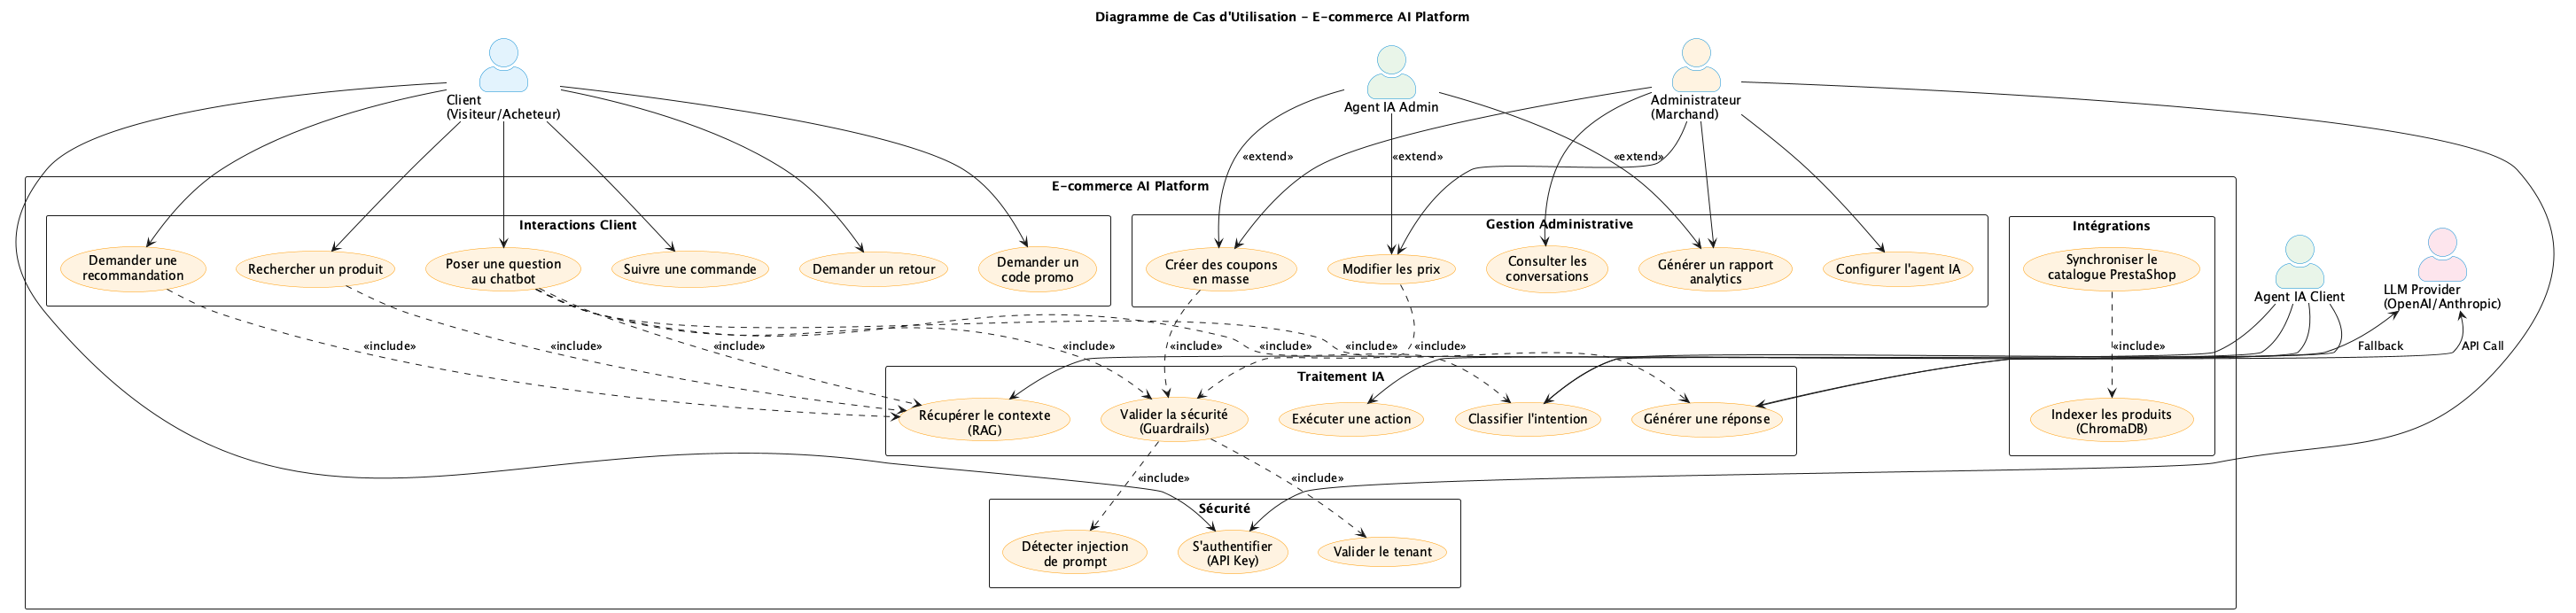
\includegraphics[width=\textwidth]{../diagrams/UseCase_Ecommerce_AI_Platform.png}
    \caption{Diagramme de cas d'utilisation de la plateforme}
    \label{fig:usecase}
\end{figure}

\section{Backlog produit}

Le \cref{tab:backlog} présente le backlog produit constitué à l'issue de la phase d'analyse, exprimé sous forme d'\emph{epics}. Chaque \emph{epic} a été décomposée en \emph{user stories} au moment de la planification du sprint correspondant (voir \cref{chap:realisation}).

\begin{table}[h]
\centering
\caption{Backlog produit (epics, par ordre de priorité)}
\label{tab:backlog}
\begin{tabular}{@{}p{0.5cm}p{6cm}p{6.5cm}@{}}
\toprule
\textbf{\#} & \textbf{Epic} & \textbf{Valeur métier} \\
\midrule
1 & Fondations techniques (infrastructure, modèles de données, synchronisation catalogue) & Prérequis à toute fonctionnalité \\
2 & Chat conversationnel augmenté (RAG) & C\oe{}ur de la proposition de valeur produit \\
3 & Sécurité, multi-tenance et supervision & Condition de mise en production \\
4 & Backoffice -- socle (tableau de bord, agent IA -- première version) & Autonomie de l'administrateur \\
5 & Moteur de règles métier \& agent IA d'administration sécurisé & Personnalisation sans intervention technique \\
6 & Analytique réelle \& finalisation backoffice & Confiance dans les données présentées \\
\bottomrule
\end{tabular}
\end{table}

\section*{Conclusion}
\addcontentsline{toc}{section}{Conclusion}

L'analyse menée dans ce chapitre a permis de traduire la problématique du stage en besoins concrets, priorisés sous forme de backlog. Le chapitre suivant détaille la conception technique retenue pour répondre à ces besoins.

\chapter{Conception}
\label{chap:conception}

\section*{Introduction}
\addcontentsline{toc}{section}{Introduction}

Ce chapitre présente les choix de conception retenus pour répondre aux besoins identifiés au chapitre précédent : architecture générale du système, choix technologiques, puis modélisation détaillée (classes, séquences) des mécanismes centraux de la plateforme.

\section{Architecture générale}

Contrairement à une architecture en microservices distincts que l'on aurait pu envisager \emph{a priori} pour un tel système, la plateforme est conçue comme un \textbf{monolithe applicatif unique} (\emph{ai-core}) exposant l'ensemble des fonctionnalités métier via une API REST, consommé exclusivement par le backoffice. Ce choix, hérité de la version initiale du projet et confirmé pendant la phase de conception, se justifie par la taille de l'équipe (un stagiaire) et par la simplicité opérationnelle qu'il procure : un seul processus à déployer et à superviser, une seule base de données à administrer, sans les coûts de coordination (cohérence transactionnelle inter-services, observabilité distribuée) qu'imposerait une décomposition en microservices à ce stade de maturité du produit.

Le \emph{ai-core} est le \textbf{seul composant autorisé à accéder directement à la base de données PostgreSQL} : cette contrainte est imposée par l'architecture (le backoffice ne détient aucun identifiant de connexion à cette base) et non laissée à la seule discipline des développeurs. Le backoffice Laravel/Filament, à l'inverse, n'a d'autre moyen d'obtenir ou de modifier une donnée que d'appeler l'API REST du \emph{ai-core}.

\begin{figure}[h]
    \centering
    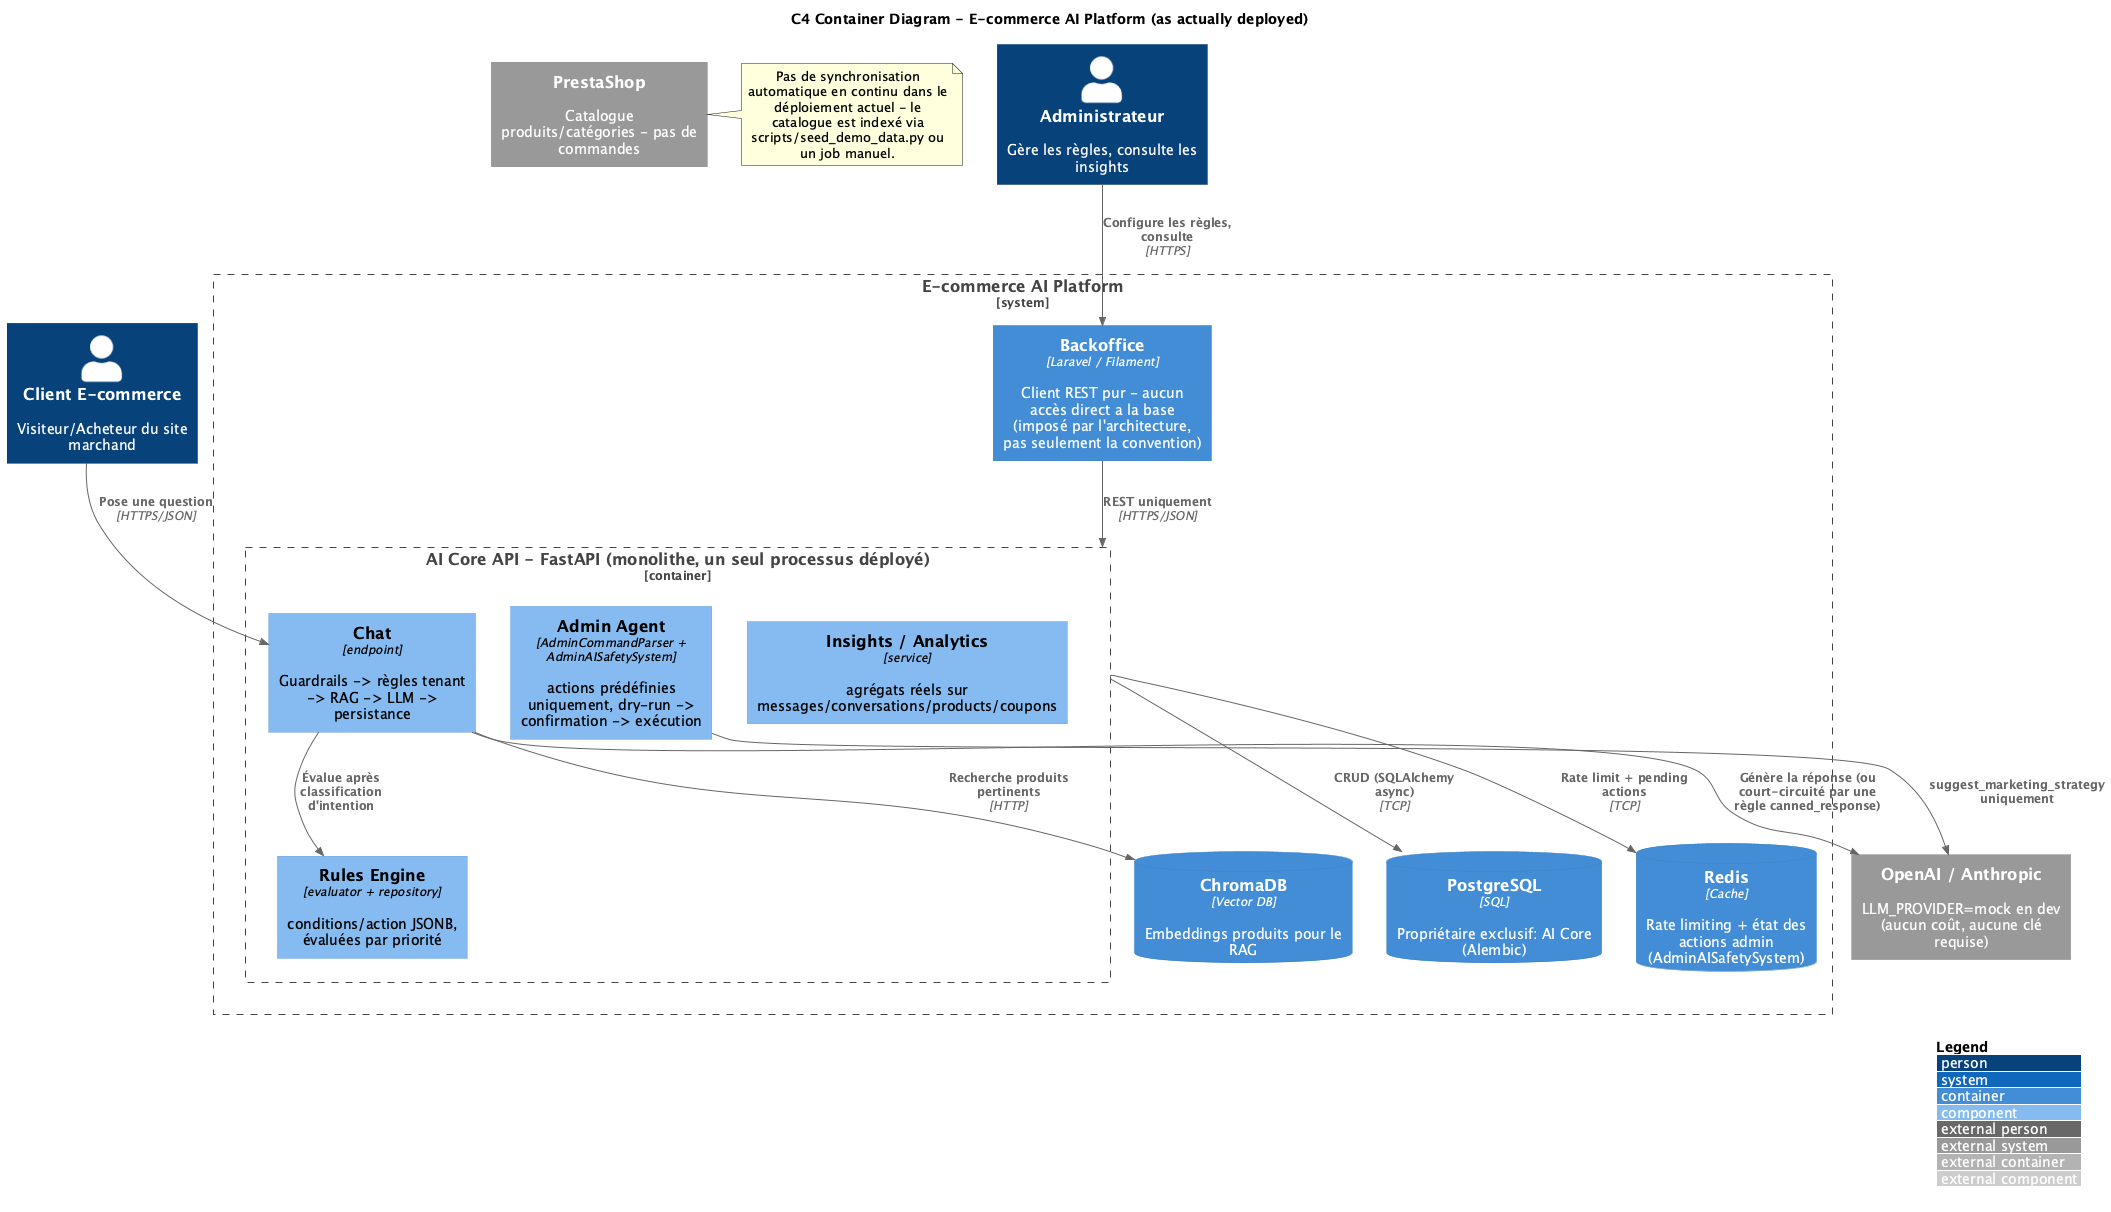
\includegraphics[width=\textwidth]{../diagrams/C4_Container.png}
    \caption{Diagramme de conteneurs (C4, niveau 2) de la plateforme}
    \label{fig:c4-container}
\end{figure}

Comme l'illustre la \cref{fig:c4-container}, quatre composants internes structurent le \emph{ai-core} : le \textbf{chat} (orchestration garde-fous -> règles -> RAG -> LLM -> persistance), le \textbf{moteur de règles}, l'\textbf{agent d'administration}, et le service d'\textbf{analyse de la demande} (\emph{insights}). Trois dépendances externes complètent l'architecture : \textbf{PostgreSQL} (persistance relationnelle, propriété exclusive du \emph{ai-core}), \textbf{ChromaDB} (base vectorielle pour la recherche sémantique de produits) et \textbf{Redis} (limitation de débit et état des actions d'administration en attente de confirmation).

\section{Choix technologiques}

\begin{table}[h]
\centering
\caption{Principaux choix technologiques}
\label{tab:stack}
\begin{tabular}{@{}p{3.5cm}p{4cm}p{6.5cm}@{}}
\toprule
\textbf{Composant} & \textbf{Technologie} & \textbf{Justification} \\
\midrule
API backend & Python 3 / FastAPI & Framework asynchrone performant, typage fort via Pydantic, génération automatique du schéma OpenAPI \\
Accès aux données & SQLAlchemy 2.0 (async) + Alembic & ORM mature avec support natif de l'asynchrone, migrations versionnées \\
Base relationnelle & PostgreSQL & Support natif du type JSONB, utilisé pour les conditions/actions des règles et les métadonnées des messages \\
Recherche sémantique & ChromaDB & Base vectorielle simple à opérer en conteneur, suffisante pour un catalogue produits de taille modérée \\
Cache / état transitoire & Redis & Nécessaire pour que l'état des actions d'administration en attente de confirmation survive aux redémarrages et soit partagé entre workers \\
Backoffice & Laravel 13 / Filament 3 & Productivité élevée pour construire une interface d'administration (CRUD, tableaux de bord) sans développer un frontend dédié \\
Interactivité backoffice & Livewire 3 & Composants réactifs côté serveur, cohérent avec l'écosystème Filament \\
Conteneurisation & Docker / Docker Compose & Environnement de développement reproductible, aligné sur le déploiement cible \\
Intégration continue & GitHub Actions & Exécution automatisée des tests et de l'analyse de qualité à chaque évolution \\
\bottomrule
\end{tabular}
\end{table}

\section{Modélisation du domaine}

Le diagramme de classes de la \cref{fig:class-diagram} présente les principales classes du système, regroupées par responsabilité : les entités du domaine persistées en base, le moteur de règles, l'agent d'administration, le service d'analyse de la demande, la couche de sécurité et l'infrastructure (fournisseurs de modèle de langage, recherche vectorielle, unité de travail transactionnelle).

\begin{figure}[h]
    \centering
    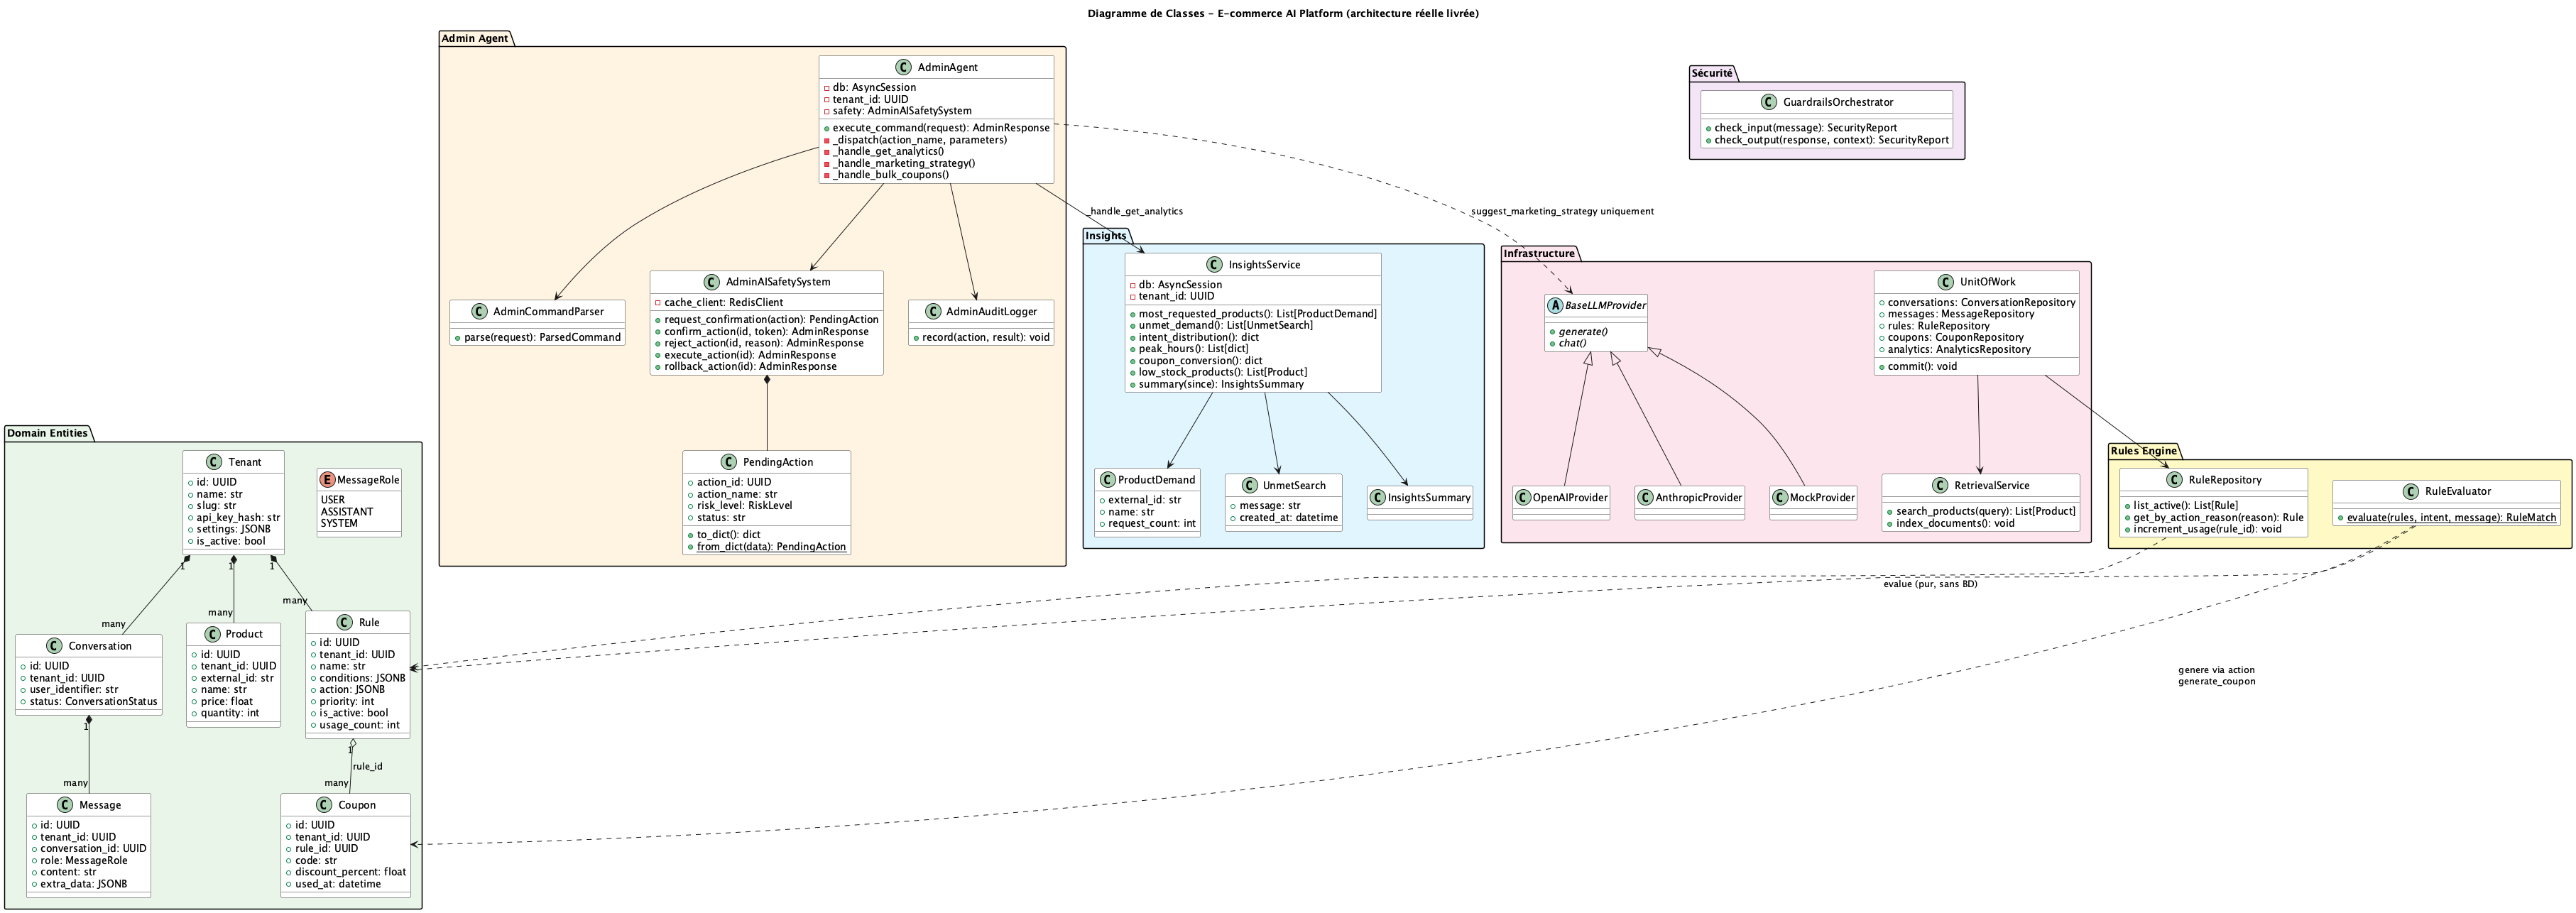
\includegraphics[width=\textwidth]{../diagrams/Class_Diagram.png}
    \caption{Diagramme de classes de la plateforme}
    \label{fig:class-diagram}
\end{figure}

Deux choix de conception méritent d'être détaillés, car ils ont directement découlé des contraintes identifiées au chapitre précédent.

\subsection{Le moteur de règles}

Le moteur de règles repose sur la séparation stricte entre \textbf{accès aux données} (\texttt{RuleRepository}, qui charge les règles actives d'un tenant, triées par priorité) et \textbf{évaluation} (\texttt{RuleEvaluator}, une fonction pure sans accès base de données ni effet de bord). Une règle est définie par des \emph{conditions} (intention détectée, présence d'au moins un mot-clé parmi une liste, ou présence de tous les mots-clés d'une liste) et une \emph{action} de l'un des trois types suivants : \texttt{canned\_response} (réponse préétablie, court-circuitant l'appel au modèle de langage), \texttt{inject\_instruction} (instruction ajoutée au contexte système envoyé au modèle) ou \texttt{generate\_coupon} (génération d'un coupon réel après la réponse). Le détail de ce mécanisme est illustré au \cref{chap:realisation} par le diagramme d'activités de la \cref{fig:rules-flow}.

Cette séparation permet de tester exhaustivement la logique de correspondance des règles sans base de données (voir \cref{chap:tests}), tout en gardant la persistance et les effets de bord (incrémentation du compteur d'utilisation, génération du coupon) dans la couche appelante.

\subsection{L'agent IA d'administration}

Le choix le plus structurant de ce chapitre concerne l'agent d'administration. Une architecture préexistante mais jamais réellement instanciée proposait un agent générique (\texttt{BaseAgent}) reposant sur des services partagés (\texttt{LLMGateway}, \texttt{RAGService}) eux-mêmes non testés et dépourvus de tout mode simulé, ce qui rendait cette voie coûteuse à finaliser sans bénéfice architectural clair. La décision retenue -- après comparaison explicite des deux options avec l'encadrant -- a été de \textbf{reconstruire l'agent d'administration sur les briques déjà éprouvées du système} : le fournisseur de modèle de langage utilisé par le chat (Groq, sans mode simulé -- les tests automatisés s'appuient sur un double de test isolé, jamais atteignable en développement ou en production), le service d'analyse de la demande, et un système de sécurité dédié.

Ce système de sécurité, \texttt{AdminAISafetySystem}, restreint l'agent à un ensemble fermé d'actions prédéfinies (\texttt{ACTION\_DEFINITIONS}), chacune associée à un niveau de risque (faible, moyen, élevé, critique) déterminant le circuit de validation requis : simple confirmation pour un risque moyen, double confirmation avec délai obligatoire pour un risque élevé, mise en file d'attente d'approbation humaine pour un risque critique. Ce workflow -- exécution à blanc (\emph{dry-run}), confirmation, exécution, annulation -- est illustré en détail par le diagramme de séquence de la \cref{fig:seq-admin-coupon}, pris sur l'exemple concret de la génération de coupons en masse.

\begin{figure}[h]
    \centering
    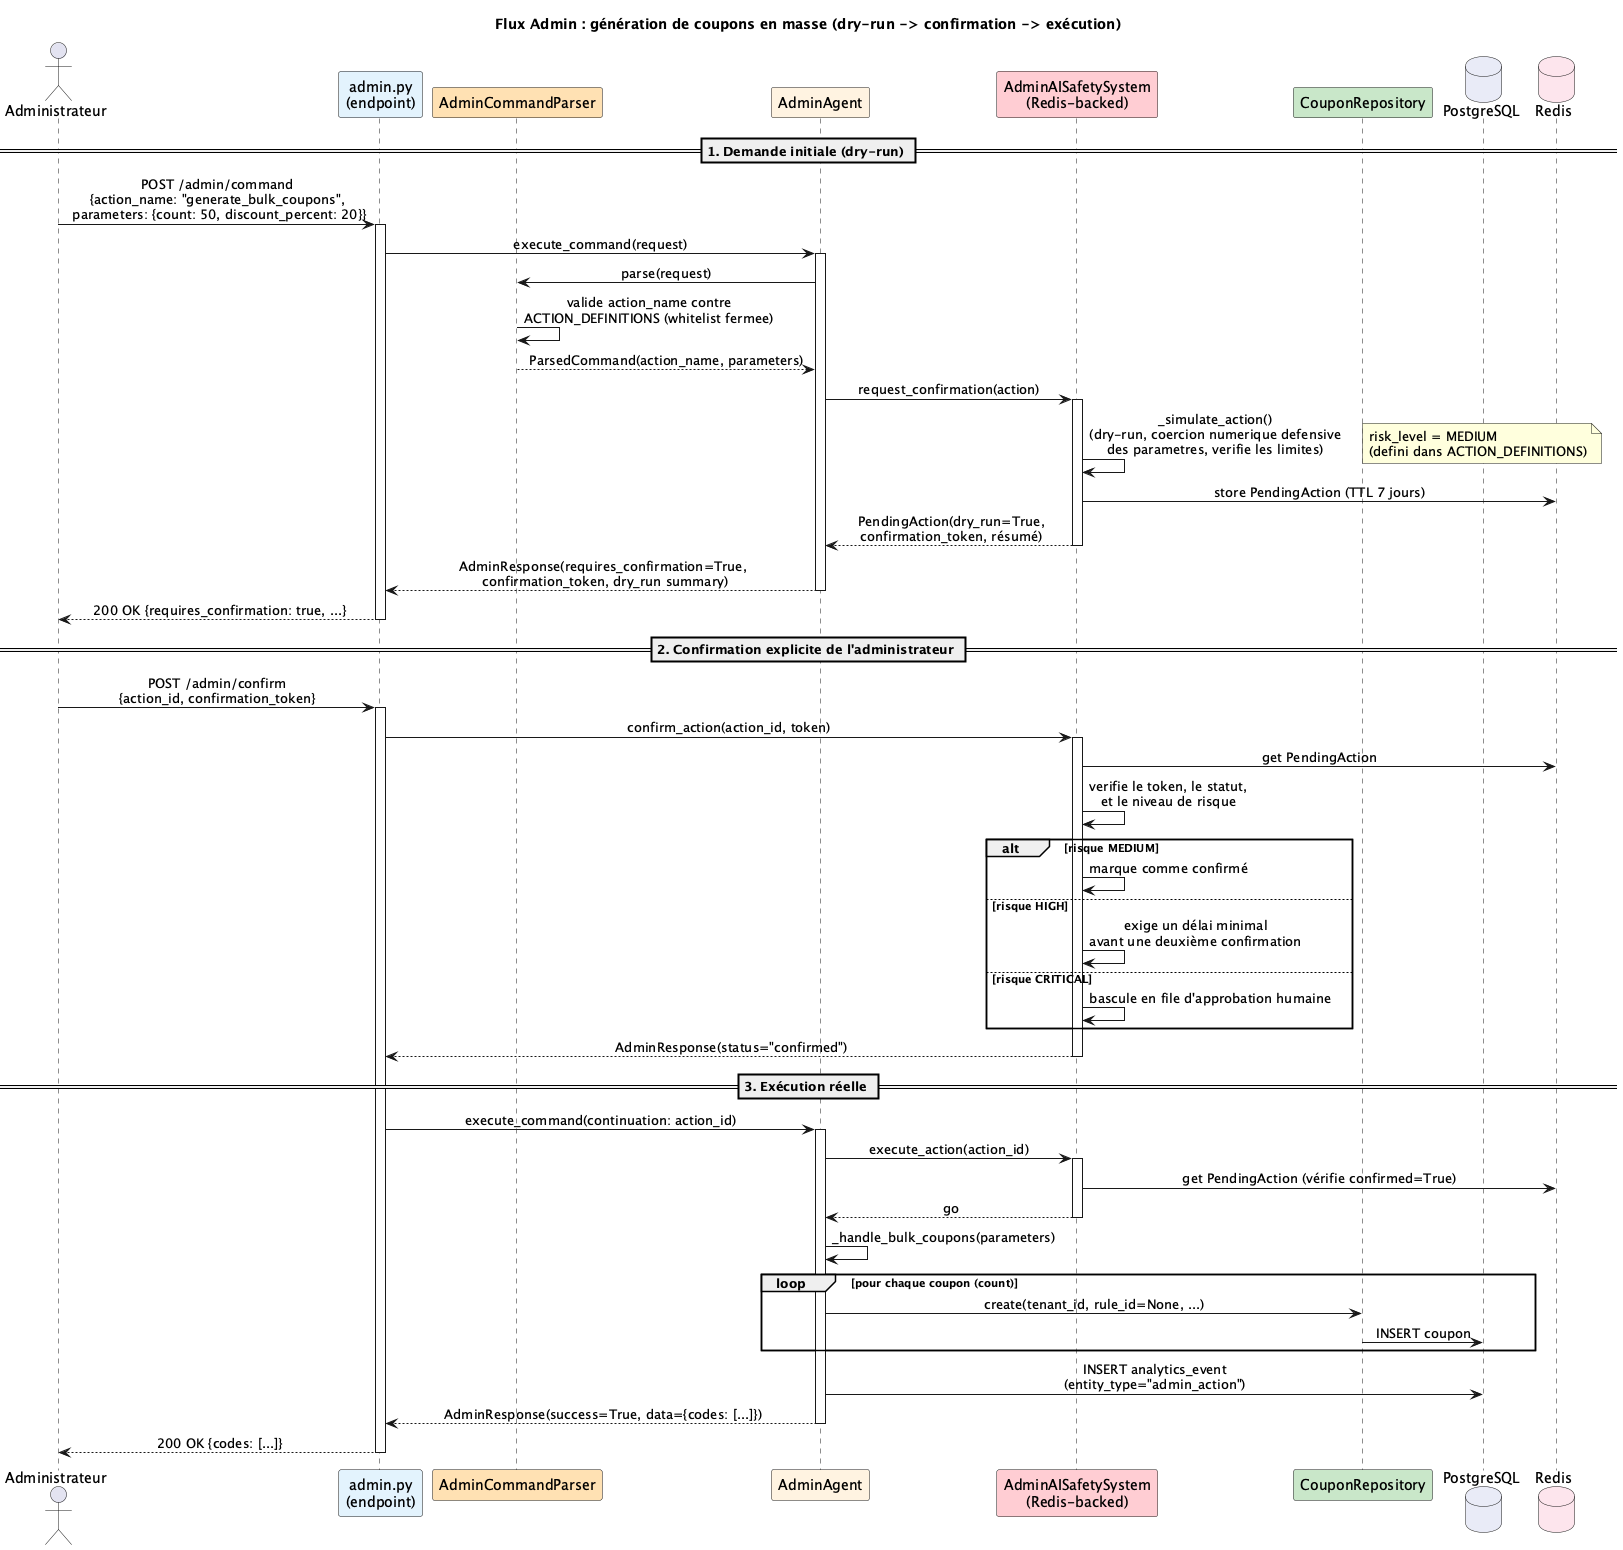
\includegraphics[width=\textwidth]{../diagrams/Sequence_Admin_Coupon.png}
    \caption{Séquence : génération de coupons en masse par l'agent d'administration}
    \label{fig:seq-admin-coupon}
\end{figure}

Point de conception notable : l'état des actions en attente de confirmation devait initialement être porté par Redis, mais l'implémentation héritée le maintenait en réalité dans un simple dictionnaire Python en mémoire -- ce qui aurait rendu toute confirmation invalide après un redémarrage du service, ou incohérente entre plusieurs \emph{workers} applicatifs. Ce point a été corrigé pendant la phase de réalisation (voir \cref{chap:realisation}, Sprint 5) en implémentant le stockage réel dans Redis, avec dégradation explicite en mémoire lorsqu'aucun client de cache n'est fourni (utile pour les tests unitaires existants).

\section{Séquence du chat conversationnel}

La \cref{fig:seq-chat} détaille le cheminement complet d'un message client, de sa réception à la persistance de la réponse : validation par les garde-fous de sécurité en entrée, classification de l'intention, évaluation des règles métier du tenant, puis -- selon le résultat -- court-circuit par une réponse préétablie, ou poursuite vers la recherche vectorielle de produits (RAG), l'appel au modèle de langage et la validation des garde-fous en sortie.

\begin{figure}[h]
    \centering
    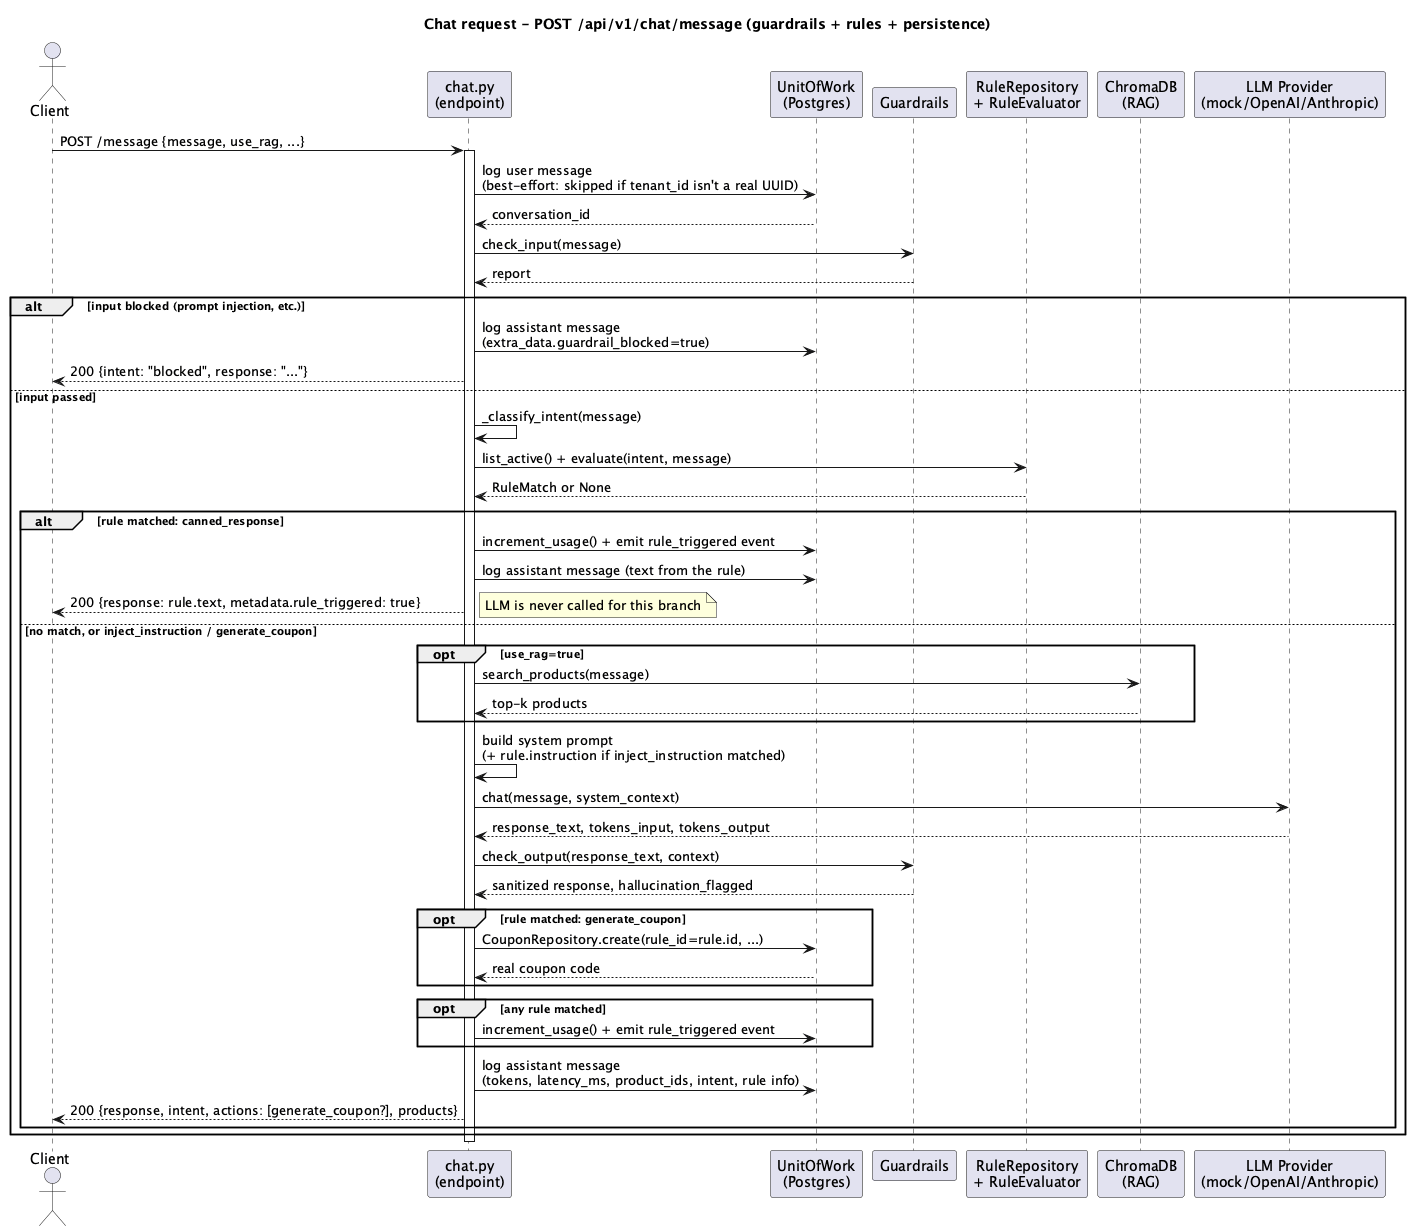
\includegraphics[width=\textwidth]{../diagrams/Sequence_Chat.png}
    \caption{Séquence complète d'une requête de chat}
    \label{fig:seq-chat}
\end{figure}

\section*{Conclusion}
\addcontentsline{toc}{section}{Conclusion}

Ce chapitre a présenté l'architecture retenue pour la plateforme ainsi que la modélisation des mécanismes centraux du système. Le chapitre suivant décrit la réalisation de ces éléments, sprint par sprint.

\chapter{Réalisation}
\label{chap:realisation}

\section*{Introduction}
\addcontentsline{toc}{section}{Introduction}

Ce chapitre détaille la phase de réalisation du projet, organisée en six sprints de deux semaines (cf. \cref{tab:planification}). Pour chaque sprint sont présentés les objectifs, le contenu livré et, le cas échéant, les difficultés rencontrées.

\section{Sprint 1 -- Fondations et infrastructure}

\subsection*{Objectifs}
Mettre en place l'environnement de développement conteneurisé, le socle de données du domaine, et la connexion en lecture au catalogue PrestaShop.

\subsection*{Réalisation}

Le sprint a débuté par la mise en place de l'\textbf{infrastructure Docker Compose} regroupant l'ensemble des services de la plateforme (\emph{ai-core}, backoffice, PostgreSQL, Redis, ChromaDB, Prometheus, Grafana), ainsi que le pipeline d'\textbf{intégration continue} sur GitHub Actions et les \textbf{migrations Alembic} versionnant le schéma de base de données.

Les \textbf{modèles de données du domaine} ont été implémentés : \texttt{Tenant} (isolation multi-tenant), \texttt{Conversation} et \texttt{Message} (historique du chat), \texttt{Product} (catalogue) et \texttt{Coupon}. La configuration PostgreSQL a été durcie (variables d'environnement sécurisées, taille de pool de connexions configurable, \emph{healthchecks} de conteneur).

Enfin, un \textbf{client PrestaShop asynchrone} a été développé (couvert par 33 tests unitaires), ainsi qu'un \textbf{service de synchronisation de catalogue} multi-tenant réalisant un \emph{upsert} en masse des produits, avec indexation vers ChromaDB optimisée par pagination en flux continu et évitement des ré-indexations inutiles par comparaison de hachage de contenu.

\section{Sprint 2 -- Moteur de chat IA}

\subsection*{Objectifs}
Livrer le c\oe{}ur fonctionnel du chat conversationnel : recherche augmentée par récupération de contexte (RAG) et orchestration de bout en bout de la réponse.

\subsection*{Réalisation}

La \textbf{recherche vectorielle de produits} (RAG) a été intégrée à l'endpoint de chat, avec prise en charge du contexte multi-tenant et repli explicite (réponse générique, sans blocage) lorsque la recherche ne retourne aucun résultat pertinent. Le patron \textbf{Unit of Work} a été mis en place pour garantir qu'une conversation entière (persistance du message utilisateur, de la réponse, des métadonnées associées) s'exécute dans une transaction cohérente. Le service d'orchestration du chat (\texttt{ChatService}) a été finalisé avec une logique d'idempotence permettant de court-circuiter le traitement d'une requête déjà traitée, ainsi que des garanties de sécurité vis-à-vis des accès concurrents sur une même conversation.

\section{Sprint 3 -- Sécurité, multi-tenance et supervision}

\subsection*{Objectifs}
Fiabiliser la plateforme avant montée en charge réelle : sécurité applicative, isolation multi-tenant, observabilité, et correction des dysfonctionnements découverts lors des tests d'intégration approfondis.

\subsection*{Réalisation}

Ce sprint a été marqué par la découverte, via des tests d'intégration plus poussés que ceux existants jusqu'alors, de plusieurs écarts significatifs entre le comportement attendu du système et son comportement réel :

\begin{itemize}
    \item les \textbf{garde-fous de sécurité} (\texttt{GuardrailsOrchestrator}, détection d'injection de prompt, masquage de données personnelles) existaient dans le code mais n'étaient \textbf{pas effectivement appelés} par l'endpoint de chat en production -- ils ont été câblés dans le chemin réel de traitement d'un message ;
    \item la \textbf{limitation de débit} (\emph{rate limiting}) était silencieusement désactivée sur l'ensemble des routes ;
    \item l'\textbf{authentification par clé API} des tenants ne fonctionnait pas de bout en bout et a dû être corrigée pour être réellement opérante ;
    \item une \textbf{faille de contournement d'authentification} a été identifiée dans le middleware de résolution du tenant et corrigée en priorité ;
    \item la \textbf{persistance des conversations et des messages}, pourtant présente dans le code depuis le sprint 2, ne s'exécutait en réalité jamais dans certains chemins -- aucune conversation n'était donc durablement enregistrée. Le défaut a été isolé et corrigé, de même que plusieurs points d'entrée laissés à l'état d'ébauche (historique de conversation, retour utilisateur, clôture de conversation).
\end{itemize}

Ces corrections, bien que non prévues telles quelles dans le backlog initial, ont été traitées en priorité dès leur découverte : elles conditionnaient la fiabilité de toute fonctionnalité construite par la suite. Le sprint s'est conclu par la mise en place du \textbf{supervisionnement applicatif} (métriques Prometheus, tableaux de bord Grafana), la correction de plusieurs métriques instrumentées mais jamais alimentées (compteurs de coût et de tokens du modèle de langage, score de confiance des réponses, panneaux d'alerte affichant systématiquement l'absence de donnée), ainsi que par la résolution de treize vulnérabilités logicielles (CVE) détectées par l'analyse de dépendances, et la mise en place d'une analyse de qualité de code continue (SonarCloud).

\section{Sprint 4 -- Backoffice Laravel/Filament : socle}

\subsection*{Objectifs}
Construire le socle du backoffice d'administration : structure de l'application Filament, client REST vers l'API \emph{ai-core}, premières pages d'administration.

\subsection*{Réalisation}

L'application \textbf{Laravel 13 / Filament 3} a été initialisée, avec un client REST dédié (\texttt{AiCoreClient}) constituant le \textbf{seul point d'accès} du backoffice vers l'API \emph{ai-core} -- aucune autre classe de l'application n'effectue d'appel HTTP direct vers ce service, ce qui centralise la gestion des erreurs réseau et la dégradation en cas d'indisponibilité. Un premier tableau de bord et une première version de la page \emph{Agent IA Admin} ont été livrés, ainsi qu'une page de paramétrage du tenant.

L'intégration avec PrestaShop a été complétée côté marchand par un \textbf{module réel} embarquant un widget de chat IA directement sur le site marchand. Plusieurs anomalies bloquantes ont été corrigées pendant ce sprint, notamment un \textbf{scénario de verrouillage total et systématique} du panneau d'administration (l'administrateur perdait l'accès au backoffice dans une situation reproductible à 100~\%), des erreurs HTTP 403 intermittentes liées à la configuration de session, ainsi que l'activation du mode \emph{WAL} de SQLite pour supporter des accès concurrents lors des tests automatisés.

\section{Sprint 5 -- Moteur de règles et agent IA d'administration sécurisé}

\subsection*{Objectifs}
Livrer les deux fonctionnalités centrales du stage : le moteur de règles métier permettant de configurer le chat sans redéploiement, et la refonte de l'agent IA d'administration sur des bases réelles et sécurisées.

\subsection*{Réalisation}

\paragraph{Moteur de règles.} Le modèle \texttt{Rule}, préexistant dans le schéma de base de données mais jamais exploité, a été relié au flux de traitement du chat. L'évaluation des règles (\texttt{RuleEvaluator}) a été implémentée comme une fonction pure, testée unitairement de façon exhaustive (voir \cref{chap:tests}), puis intégrée dans l'endpoint de chat juste après la classification d'intention : en cas de correspondance, l'action associée (réponse préétablie, instruction injectée, génération de coupon) est appliquée selon le mécanisme détaillé à la \cref{fig:rules-flow}. Une interface complète de gestion des règles (création, modification, suppression) a été exposée côté API puis côté backoffice. La politique de remise historiquement codée en dur dans le service de coupons a été repliée dans ce même mécanisme de règles, avec conservation d'une valeur par défaut en l'absence de règle applicable.

\begin{figure}[h]
    \centering
    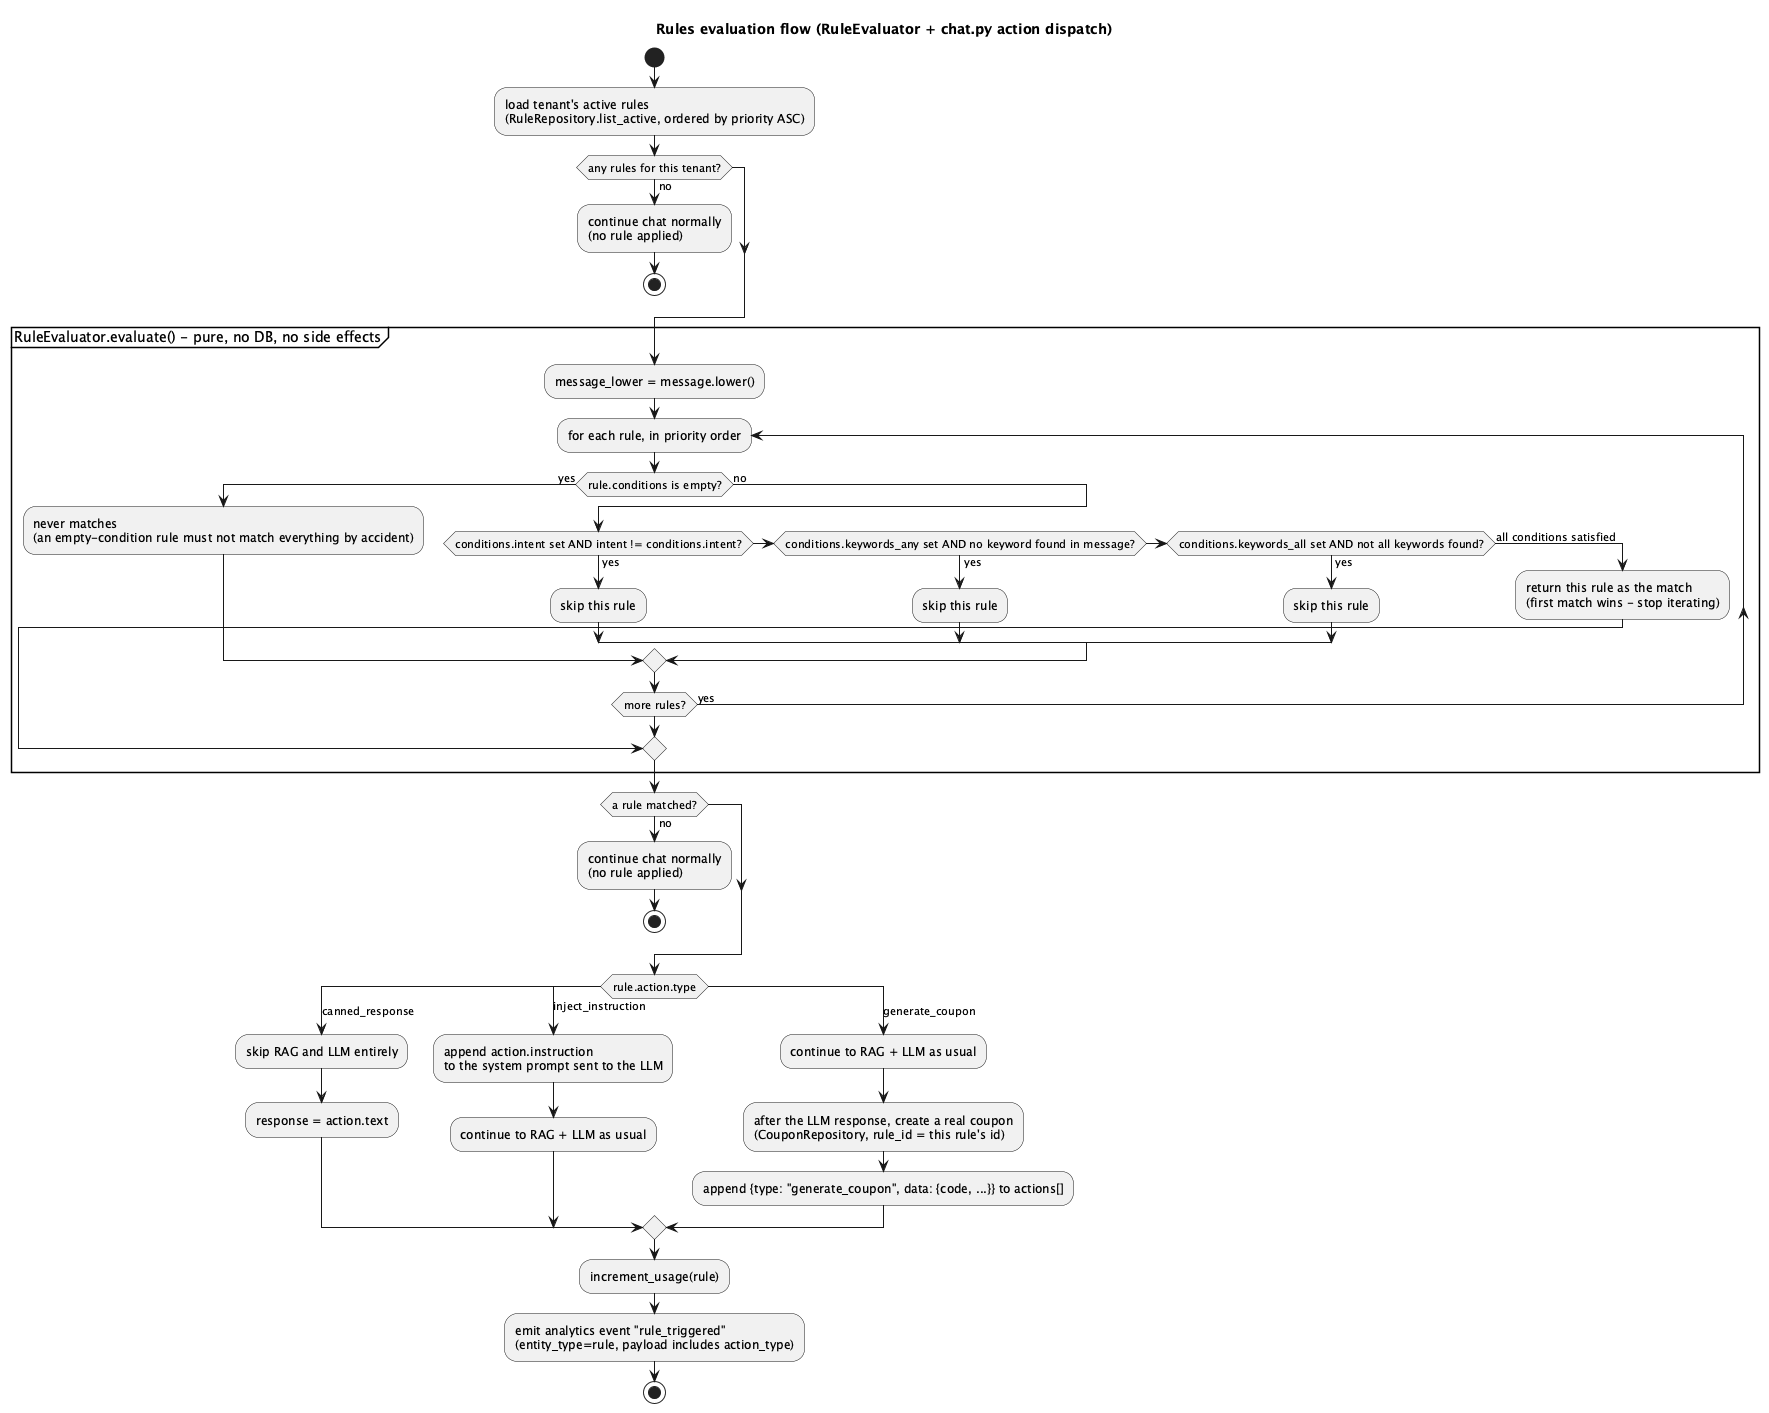
\includegraphics[width=0.9\textwidth]{../diagrams/Rules_Evaluation_Flow.png}
    \caption{Diagramme d'activités : évaluation des règles et répartition des actions}
    \label{fig:rules-flow}
\end{figure}

\paragraph{Agent IA d'administration.} Conformément au choix de conception exposé au \cref{chap:conception}, l'agent d'administration a été entièrement reconstruit. Un analyseur de commandes (\texttt{AdminCommandParser}) restreint désormais l'agent à un ensemble fermé d'actions prédéfinies, qu'elles soient exprimées de façon structurée ou en langage naturel (classification par mots-clés). Le système de sécurité (\texttt{AdminAISafetySystem}) a été effectivement adossé à Redis -- corrigeant un écart entre la documentation du composant, qui annonçait un état persistant, et son implémentation réelle, qui le maintenait jusque-là en mémoire locale du processus.

Les données présentées par l'agent (statistiques, produits en demande, demande non satisfaite) ont été entièrement reconstruites à partir du nouveau service \texttt{InsightsService}, remplaçant des valeurs d'exemple fixes (chiffre d'affaires fictif, noms de produits génériques) par des agrégats calculés sur les messages, conversations, produits et coupons réellement enregistrés. Un défaut a été détecté lors des essais manuels de l'interface d'administration reconstruite : les paramètres saisis via le formulaire du backoffice étant systématiquement transmis sous forme de chaînes de caractères, une comparaison numérique effectuée lors de la simulation d'une action (\emph{dry-run}) provoquait une erreur de type non gérée. Ce défaut a été corrigé par une coercition défensive des paramètres numériques, et une régression a été ajoutée à la suite de tests pour empêcher sa réintroduction.

\section{Sprint 6 -- Finalisation du backoffice et documentation}

\subsection*{Objectifs}
Achever l'exposition, côté backoffice, des fonctionnalités livrées au sprint précédent, et mettre à jour la documentation du projet en fin de stage.

\subsection*{Réalisation}

Le tableau de bord du backoffice a été doté de \textbf{graphiques réels} (Chart.js), alimentés par un nouvel endpoint d'API dédié aux séries temporelles, remplaçant les graphiques statiques initiaux. Une page \emph{Coûts \& Messages} a été ajoutée pour le suivi de la consommation du modèle de langage (tokens, coût, latence moyenne, messages les plus coûteux), ainsi qu'un navigateur de conversations permettant de consulter l'historique complet des échanges d'un tenant, et une page \emph{Insights} restituant l'ensemble des indicateurs de demande calculés par le service dédié.

L'interface de l'agent IA d'administration, jugée initialement trop rudimentaire (un simple formulaire de sélection d'action), a été retravaillée en une véritable \textbf{interface de type conversation}, conservant l'historique des échanges dans la session et présentant chaque résultat (statistiques, propositions de stratégie marketing, codes de coupons générés) sous une forme visuelle adaptée à sa nature plutôt qu'en JSON brut. Un défaut d'expérience utilisateur a également été corrigé sur les graphiques de répartition des intentions : en l'absence de toute donnée sur la période sélectionnée, un graphique vide s'affichait sans distinction visuelle avec un graphique en échec technique ; un état vide explicite a été introduit.

Le sprint s'est conclu par la consolidation de la documentation du projet : réécriture du \texttt{README}, mise à jour des diagrammes d'architecture pour refléter le système effectivement livré plutôt que sa conception initiale, et export automatisé du schéma \texttt{OpenAPI} de l'API depuis l'application elle-même, garantissant sa cohérence avec le code réel.

\section*{Conclusion}
\addcontentsline{toc}{section}{Conclusion}

Ce chapitre a détaillé, sprint par sprint, la réalisation du projet. Le chapitre suivant présente la démarche de tests et de validation mise en \oe{}uvre pour garantir la fiabilité de l'ensemble.

\chapter{Tests et validation}
\label{chap:tests}

\section*{Introduction}
\addcontentsline{toc}{section}{Introduction}

Ce chapitre présente la démarche de tests mise en \oe{}uvre tout au long du projet, ainsi que les résultats obtenus sur la version finale livrée. Conformément à la \emph{definition of done} adoptée dès le premier sprint (\cref{chap:cadre-general}), aucune fonctionnalité n'a été considérée terminée sans couverture de test correspondante.

\section{Stratégie de tests}

Trois niveaux de tests ont été mis en \oe{}uvre, chacun avec un objectif distinct.

\subsection{Tests unitaires}

Les tests unitaires couvrent la logique pure, sans dépendance externe (base de données, cache, réseau). C'est en particulier le cas de l'évaluateur de règles (\texttt{RuleEvaluator}), testé à l'aide d'objets de substitution légers plutôt que de véritables enregistrements en base, ce qui permet une exécution rapide et déterministe. Treize scénarios y sont couverts : correspondance sur l'intention, sur un mot-clé parmi plusieurs, sur l'ensemble de mots-clés requis, absence de correspondance, priorité entre règles concurrentes, et le cas limite d'une règle sans aucune condition (qui, par construction, ne doit jamais correspondre par accident).

\subsection{Tests d'intégration}

Les tests d'intégration s'exécutent contre une véritable instance PostgreSQL (ignorés automatiquement si aucune instance n'est joignable, pour ne pas bloquer un environnement de développement incomplet) et valident des scénarios de bout en bout via de véritables appels HTTP à l'application. C'est à ce niveau qu'ont été validés, par exemple : la création réelle d'un coupon en base par une règle de type \texttt{generate\_coupon}, l'incrémentation du compteur d'utilisation d'une règle après plusieurs déclenchements, le court-circuit effectif du modèle de langage par une réponse préétablie (vérifié à l'aide d'un fournisseur de modèle de langage instrumenté, garantissant qu'il n'est jamais sollicité dans ce cas), les trois paliers de risque du système de sécurité de l'agent d'administration, ou encore l'exactitude des indicateurs du service d'analyse de la demande sur un jeu de données de test dont le résultat attendu est calculé manuellement puis comparé à la valeur produite par le système.

\subsection{Tests applicatifs (backoffice)}

Côté backoffice, les tests s'appuient sur le simulateur HTTP de Laravel pour isoler chaque page Filament de l'API réelle (réponses simulées), et vérifient à la fois le comportement nominal et la dégradation gracieuse en cas d'indisponibilité du \emph{ai-core} (page fonctionnelle affichant un message d'erreur plutôt qu'une erreur fatale).

\subsection{Vérification manuelle}

Les tests automatisés ne suffisant pas à eux seuls à garantir la qualité perçue d'une interface, chaque page du backoffice a par ailleurs été vérifiée manuellement en conditions réelles : démarrage de la pile applicative complète, injection de données de test représentatives via l'API, puis inspection visuelle du rendu. Cette étape a permis de détecter des défauts qu'aucun test automatisé n'aurait révélés : une erreur de type sur un paramètre transmis sous forme de chaîne par un formulaire (\cref{chap:realisation}, Sprint 5), ou l'absence de distinction visuelle entre un graphique légitimement vide et un graphique en échec (Sprint 6).

\section{Résultats}

\begin{table}[h]
\centering
\caption{Synthèse de la couverture de tests à la livraison finale}
\label{tab:tests-resultats}
\begin{tabular}{@{}p{5cm}p{3cm}p{6cm}@{}}
\toprule
\textbf{Composant} & \textbf{Tests passants} & \textbf{Outils} \\
\midrule
\emph{ai-core} (Python) & 563 & pytest (unitaires + intégration) \\
Backoffice (PHP) & 36 & PHPUnit / Livewire testing \\
\bottomrule
\end{tabular}
\end{table}

Au-delà des tests fonctionnels, chaque livraison a été systématiquement validée par les outils d'analyse statique du projet : \texttt{ruff check} et \texttt{ruff format --check} côté Python, \texttt{pint --test} (respect des conventions de style Laravel) côté PHP -- les deux exécutés sans erreur sur la version finale.

\section{Exemple : validation du calcul de la demande non satisfaite}

Un exemple illustre la rigueur recherchée dans les tests d'intégration : le calcul de la \emph{demande non satisfaite} (recherches client n'ayant renvoyé aucun résultat produit pertinent) nécessitait d'associer chaque réponse infructueuse de l'assistant au message utilisateur qui l'avait précédée. Une première implémentation, fondée sur un rapprochement par proximité temporelle, s'est révélée non déterministe en cas de messages horodatés de façon identique lors des tests. Le calcul a été repensé pour s'appuyer sur l'invariant réel du système -- chaque message utilisateur est immédiatement suivi de la réponse de l'assistant dans le même flux de traitement -- en associant chaque paire par rang au sein de la conversation plutôt que par horodatage, rendant le résultat déterministe et vérifiable par un test d'intégration exact.

\section*{Conclusion}
\addcontentsline{toc}{section}{Conclusion}

La démarche de tests mise en place a permis de livrer une version du système dont le comportement -- y compris les cas limites et les mécanismes de sécurité -- est vérifié de façon reproductible, condition jugée nécessaire au regard de la problématique de confiance posée en introduction de ce rapport.

\chapter*{Conclusion générale et perspectives}
\addcontentsline{toc}{chapter}{Conclusion générale et perspectives}
\markboth{Conclusion générale et perspectives}{}

Ce stage de fin d'études, réalisé au sein de Prodexo sur une période de six mois, avait pour objectif de faire évoluer une plateforme d'assistant IA e-commerce d'un socle technique fonctionnel vers un produit réellement exploitable par un administrateur de boutique. Cet objectif se déclinait en deux exigences complémentaires : rendre le comportement de l'assistant configurable sans intervention technique, et garantir que les informations présentées à l'administrateur reflètent fidèlement l'activité réelle du système.

Les travaux menés ont permis de livrer un \textbf{moteur de règles métier} intégré au flux de traitement du chat, un \textbf{agent IA d'administration} restreint à un ensemble d'actions prédéfinies et protégé par un workflow de confirmation adapté au niveau de risque de chaque action, un \textbf{service d'analyse de la demande client} fondé exclusivement sur des données réellement collectées, ainsi qu'un \textbf{backoffice} complet exposant l'ensemble de ces capacités. Une part substantielle de ce travail a consisté à auditer méthodiquement l'existant pour distinguer ce qui fonctionnait réellement de ce qui n'était qu'apparence -- démarche qui s'est révélée aussi formatrice que l'écriture de code neuf, et qui a mis en lumière plusieurs anomalies significatives (garde-fous de sécurité non câblés, persistance de conversations défaillante, données d'administration fabriquées) corrigées au fil des sprints.

Sur le plan personnel, ce stage a été l'occasion d'approfondir des compétences en développement backend asynchrone (FastAPI, SQLAlchemy), en conception d'API, en sécurisation de systèmes automatisés à effet réel, ainsi qu'en développement d'interfaces d'administration avec l'écosystème Laravel/Filament. Il a également permis de pratiquer une démarche de gestion de projet agile de bout en bout, de la constitution d'un backlog à la livraison itérative de sprints testés et documentés.

Plusieurs pistes d'évolution se dégagent naturellement de ce travail pour la suite du projet :

\begin{itemize}
    \item l'intégration d'une véritable table de commandes, aujourd'hui absente du système, qui permettrait d'enrichir significativement les indicateurs d'analyse (taux de conversion réel, chiffre d'affaires attribuable au chat) au-delà des seuls signaux de demande actuellement disponibles ;
    \item l'extension du moteur de règles à des conditions plus riches (segmentation client, historique d'achat) une fois cette donnée disponible ;
    \item la mise en place d'un parcours d'inscription et de facturation self-service complet pour les tenants, actuellement limité à un mode de développement ;
    \item l'industrialisation du déploiement en production, au-delà de l'environnement Docker Compose utilisé en développement.
\end{itemize}

Ce travail constitue une base solide et honnêtement documentée sur laquelle ces évolutions pourront s'appuyer.


% ----------------------------------------------------------------------------
% Annexes et bibliographie
% ----------------------------------------------------------------------------
\appendix
\chapter*{Bibliographie et Netographie}
\addcontentsline{toc}{chapter}{Bibliographie et Netographie}
\markboth{Bibliographie et Netographie}{}

\begin{thebibliography}{99}

\bibitem{scrumguide}
Schwaber, K. et Sutherland, J. \emph{The Scrum Guide}. 2020.
\url{https://scrumguides.org/}

\bibitem{fastapi}
\emph{FastAPI Documentation}. 2026.
\url{https://fastapi.tiangolo.com/}

\bibitem{sqlalchemy}
\emph{SQLAlchemy 2.0 Documentation}. 2026.
\url{https://docs.sqlalchemy.org/en/20/}

\bibitem{filament}
\emph{Filament -- Rapid Laravel Development Framework}. 2026.
\url{https://filamentphp.com/docs}

\bibitem{livewire}
\emph{Laravel Livewire Documentation}. 2026.
\url{https://livewire.laravel.com/docs}

\bibitem{chromadb}
\emph{Chroma -- The AI-native Open-source Embedding Database}. 2026.
\url{https://docs.trychroma.com/}

\bibitem{owasp-llm}
OWASP Foundation. \emph{OWASP Top 10 for Large Language Model Applications}. 2025.
\url{https://owasp.org/www-project-top-10-for-large-language-model-applications/}

\bibitem{c4model}
Brown, S. \emph{The C4 model for visualising software architecture}. 2026.
\url{https://c4model.com/}

\bibitem{prestashop-webservice}
\emph{PrestaShop Webservice API Documentation}. 2026.
\url{https://devdocs.prestashop-project.org/8/webservice/}

\bibitem{redis-docs}
\emph{Redis Documentation}. 2026.
\url{https://redis.io/docs/}

\end{thebibliography}


\chapter{Extraits de code significatifs}
\label{annexe:code}

Cette annexe présente deux extraits représentatifs, tirés tels quels du code source livré, illustrant les mécanismes centraux décrits au \cref{chap:conception}.

\section{Évaluation pure des règles métier}

L'extrait ci-dessous (\texttt{app/services/rules/evaluator.py}) montre l'implémentation du \texttt{RuleEvaluator} : une fonction sans accès à la base de données, ce qui la rend testable de façon exhaustive et rapide (voir \cref{chap:tests}).

\begin{lstlisting}[language=Python, caption={Correspondance des conditions d'une règle}]
@staticmethod
def _matches_conditions(conditions, intent, message_lower):
    if not conditions:
        return False

    known_keys = ("intent", "keywords_any", "keywords_all")
    if not any(key in conditions for key in known_keys):
        return False

    if "intent" in conditions and conditions["intent"] != intent:
        return False

    if "keywords_any" in conditions:
        keywords = [kw.lower() for kw in conditions["keywords_any"]]
        if not any(kw in message_lower for kw in keywords):
            return False

    if "keywords_all" in conditions:
        keywords = [kw.lower() for kw in conditions["keywords_all"]]
        if not all(kw in message_lower for kw in keywords):
            return False

    return True

def evaluate(self, rules, intent, message):
    """Retourne la premiere regle qui matche, ou None."""
    message_lower = message.lower()
    for rule in rules:
        if self._matches_conditions(rule.conditions or {}, intent, message_lower):
            return RuleMatch(rule=rule, action=rule.action or {})
    return None
\end{lstlisting}

Le choix explicite qu'une règle sans aucune des trois clés de condition connues ne corresponde jamais (plutôt que de matcher par défaut) évite qu'une règle mal configurée n'intercepte silencieusement l'intégralité du trafic d'un tenant.

\section{Classification des actions d'administration par niveau de risque}

L'extrait ci-dessous (\texttt{app/core/security/admin\_safety.py}) montre un sous-ensemble du registre \texttt{ACTION\_DEFINITIONS}, qui constitue la liste fermée des actions que l'agent d'administration est autorisé à exécuter. Chaque action y est associée à un niveau de risque déterminant le circuit d'approbation requis (cf. \cref{fig:seq-admin-coupon}).

\begin{lstlisting}[language=Python, caption={Extrait du registre des actions administratives autorisées}]
ACTION_DEFINITIONS: Dict[str, ActionDefinition] = {
    # RISQUE FAIBLE - execution automatique
    "get_analytics": ActionDefinition(
        name="get_analytics",
        description="Recupere les analytics (lecture seule)",
        risk_level=RiskLevel.LOW,
        approval_type=ApprovalType.NONE,
        supports_rollback=False,
    ),
    # RISQUE ELEVE - double confirmation + delai
    "generate_bulk_coupons": ActionDefinition(
        name="generate_bulk_coupons",
        description="Genere des coupons en masse",
        risk_level=RiskLevel.HIGH,
        approval_type=ApprovalType.DOUBLE,
        requires_reason=True,
        cooldown_seconds=3600,  # 1h entre deux generations en masse
    ),
    ...
}
\end{lstlisting}

Toute action absente de ce registre est rejetée par l'\texttt{AdminCommandParser} avant même d'atteindre la logique d'exécution -- l'agent ne dispose d'aucune capacité d'exécution libre.

\chapter{Dictionnaire de données}
\label{annexe:donnees}

Cette annexe présente les principales tables du schéma relationnel, propriété exclusive du service \emph{ai-core} (\cref{chap:conception}). Les colonnes techniques communes (identifiant primaire \gls{uuid}, horodatages de création/mise à jour) sont omises par souci de lisibilité lorsqu'elles ne portent pas d'information métier spécifique.

\begin{table}[h]
\centering
\caption{Table \texttt{tenants}}
\begin{tabular}{@{}p{4cm}p{11cm}@{}}
\toprule
\textbf{Colonne} & \textbf{Description} \\
\midrule
\texttt{name}, \texttt{slug} & Identité du tenant (marchand) \\
\texttt{api\_key\_hash} & Hachage de la clé d'API utilisée pour l'authentification serveur-à-serveur \\
\texttt{email}, \texttt{is\_verified}, \texttt{verification\_token\_hash} & Inscription self-service avec vérification par courriel \\
\texttt{settings} & Paramètres libres du tenant (\gls{jsonb}) \\
\texttt{is\_active} & Active ou désactive le tenant sans suppression de ses données \\
\bottomrule
\end{tabular}
\end{table}

\begin{table}[h]
\centering
\caption{Tables \texttt{conversations} et \texttt{messages}}
\begin{tabular}{@{}p{4cm}p{11cm}@{}}
\toprule
\textbf{Colonne} & \textbf{Description} \\
\midrule
\texttt{conversations.tenant\_id} & Clé étrangère vers le tenant propriétaire (isolation multi-tenant) \\
\texttt{conversations.user\_identifier} & Identifiant du client côté site marchand \\
\texttt{conversations.status} & État de la conversation (ouverte, fermée) \\
\texttt{messages.role} & \texttt{USER} / \texttt{ASSISTANT} / \texttt{SYSTEM} \\
\texttt{messages.content} & Contenu textuel du message \\
\texttt{messages.idempotency\_key} & Empêche le double traitement d'une requête réémise \\
\texttt{messages.extra\_data} & Métadonnées structurées (\gls{jsonb}) : intention détectée, produits retournés, règle éventuellement déclenchée, usage RAG \\
\texttt{messages.tokens\_input/output}, \texttt{latency\_ms} & Mesures de coût et de performance de l'appel au \gls{llm} \\
\bottomrule
\end{tabular}
\end{table}

\begin{table}[h]
\centering
\caption{Table \texttt{rules}}
\begin{tabular}{@{}p{4cm}p{11cm}@{}}
\toprule
\textbf{Colonne} & \textbf{Description} \\
\midrule
\texttt{tenant\_id} & Isolation multi-tenant \\
\texttt{name}, \texttt{description} & Libellé de la règle, affiché dans le backoffice \\
\texttt{conditions} & \gls{jsonb} -- clés supportées : \texttt{intent}, \texttt{keywords\_any}, \texttt{keywords\_all} \\
\texttt{action} & \gls{jsonb} -- type (\texttt{canned\_response} / \texttt{inject\_instruction} / \texttt{generate\_coupon}) et paramètres associés \\
\texttt{priority} & Ordre d'évaluation (croissant) entre règles concurrentes \\
\texttt{is\_active} & Permet de désactiver une règle sans la supprimer \\
\texttt{usage\_count} & Compteur de déclenchements, incrémenté à chaque correspondance \\
\bottomrule
\end{tabular}
\end{table}

\begin{table}[h]
\centering
\caption{Table \texttt{coupons}}
\begin{tabular}{@{}p{4cm}p{11cm}@{}}
\toprule
\textbf{Colonne} & \textbf{Description} \\
\midrule
\texttt{tenant\_id}, \texttt{conversation\_id} & Contexte d'émission du coupon \\
\texttt{rule\_id} & Règle à l'origine de la génération, le cas échéant (\texttt{NULL} si généré par l'agent d'administration) \\
\texttt{code} & Code promotionnel généré \\
\texttt{discount\_percent} / \texttt{discount\_amount} & Remise en pourcentage ou en valeur (centimes) \\
\texttt{status}, \texttt{used\_at} & Suivi de l'utilisation effective du coupon (base du calcul du taux de conversion, \cref{chap:conception}) \\
\texttt{expires\_at} & Date d'expiration \\
\bottomrule
\end{tabular}
\end{table}

\begin{table}[h]
\centering
\caption{Table \texttt{products}}
\begin{tabular}{@{}p{4cm}p{11cm}@{}}
\toprule
\textbf{Colonne} & \textbf{Description} \\
\midrule
\texttt{tenant\_id}, \texttt{external\_id} & Identifiant du produit côté PrestaShop \\
\texttt{name}, \texttt{description}, \texttt{category\_name}, \texttt{manufacturer\_name} & Attributs indexés pour la recherche vectorielle (RAG) \\
\texttt{price}, \texttt{quantity} & Prix et stock, synchronisés depuis PrestaShop \\
\texttt{active}, \texttt{available\_for\_order} & Disponibilité du produit \\
\bottomrule
\end{tabular}
\end{table}

\bigskip
\noindent\textbf{Remarque.} Aucune table de commandes n'existe dans ce schéma : le catalogue synchronisé depuis PrestaShop se limite aux produits et catégories. Toute métrique de conversion présentée dans le backoffice (\cref{chap:realisation}) est en conséquence dérivée d'un signal de \emph{demande} (recherches et messages du chat), et non d'un signal de \emph{vente}.


\end{document}
